\documentclass{article}

\usepackage{color}
\usepackage{graphicx}
\usepackage{amsmath}
\usepackage{indentfirst}
\usepackage{float}
\usepackage{siunitx}
\begin{document}
\vspace*{0.25cm}
\hrulefill
\thispagestyle{empty}

\begin{center}
\begin{large}
\sc{UM--SJTU Joint Institute \vspace{0.3em} \\ Ve215}
\end{large}

\hrulefill

\vspace*{5cm}
\begin{Large}
\sc{{Laboratory Report}}
\end{Large}

\vspace{2em}

\begin{large}
\sc{{Exercise 3
\vspace{0.5em}

Transient Lab}}
\end{large}
\end{center}


\vfill

\begin{table}[h!]
\flushleft
\begin{tabular}{ll}
Name: Jin Minhao \hspace*{2em}&
ID: 516370910116\hspace*{2em}\\





Date: \today

\end{tabular}
\end{table}


\newpage
\section{Introduction}
\subsection{Objectives}
\begin{enumerate}
	\item Apply the theory you learned on the step responses in first- and secondorder circuits to series RC and RLC circuits, which you will build in the lab.
	\item Build a series RC circuit, observe its responses to input square wave
	signal of varied frequency, and explain them based on the theory you learned:
	\begin{enumerate}
		\item Relate the observed capacitor voltage and resistor voltage as functions
		of time to your pre-lab calculations
		\item Explain the changes of both output waveforms in response to the
		increase of the frequency of the input square wave signal
		\item Explain the amplitudes of the capacitor voltage and the resistor voltage
		related to the amplitude of the input square wave
	\end{enumerate}
	\item Build a series RLC circuit, observe the three types of its responses to
	input square wave signal, and relate them to the theory you have learned. For
	the under-damped/ over-damped/ critical damped response, compare the
	resistance in the circuit measured in the lab with the critical resistance you
	calculated in the pre-lab.
	\item Build the simplest second-order circuit, an LC tank, and observe oscillations.
\end{enumerate}
\subsection{Theoretical Background}
\subsection{First-order circuits}
Theoretically, the transient responses in electric circuits are described by
differential equations. The circuits, whose responses obey the first-order
differ-ential equation
$$\frac{dx(x)}{dt}+\frac{1}{r}=f(t)$$
are called first-order circuits. Their responses are always monotonic and
appear in the form of exponential function
$$x(t)=K_1e^{-(\frac{t}{r})}+K_2$$
A first-order circuit includes the effective resistance R and one energystorage element, an inductor L or a capacitor C .

In an RC circuit, the time constant is
$$r=RC$$
In an LC circuit, the time constant is
$$r=\frac{L}{R}$$
The fall time of a signal is defined as the interval between the moment when
the signal reaches its 90\% and the moment when the signal reaches its 10\% level.
Note that the 10\% level is reached between $2\tau$ and $3\tau$ . Approximately, you can
assume f $alltime \approx 2.2\tau$ . After $t = 5\tau$ , the exponent practically equals zero.
\subsection{Second-order circuits}
Many circuits involve two energy-storing elements, both an inductor L and a
capacitor C . Such circuits require a second-order differential equation description
$$\frac{d^2x(t)}{dt^2}+2\alpha\frac{dx(t)}{dt}+w_0^2x(t)=f(t)$$
thus they are called second-order circuits.

We will consider only second-order circuits with one inductor and one capacitor. The differential equation includes two parameters: the damping factor
$\alpha$ and the undamped frequency $\omega_0$ which are determined by the circuit and its
components.

For example, in the series RLC circuit, which you will build and study in
this lab,
$$\alpha=\frac{R}{2L}$$ and $$\omega_0=\sqrt{\frac{1}{LC}}$$
while in the parallel RLC circuit,
$$\alpha=\frac{1}{2RC}$$ and $$\omega_0=\sqrt{\frac{1}{LC}}$$
Depending on the two parameters α$\alpha$ and $\omega_0$, second-order circuits can
exhibit three types of responses.
\subsubsection{The underdamped response}
If $\alpha <\omega_0$
$$x(t)=e^{-\alpha t}(K_1cos(\omega t)+K_2sin_\omega t)$$
where $\omega=\omega_0)^2-\alpha^2$

The underdamped circuit response involves decaying oscillations, which
may last for many periods or for less than one period, depending on the
damping ratio $\varepsilon=\frac{\alpha}{\omega_0}$, which for the series RLC circuit $\varepsilon=\frac{R}{2L}\sqrt{LC}=\frac{R}{2}\sqrt{\frac{C}{L}}$. Varying the values of R, L, C, affects the damping ratio $\varepsilon$.
\subsubsection{The critically damped response}
If $\alpha=\omega_0$
$$x(t)=e^{-\alpha t}(K_1+K_2t)$$
and the circuit has the critically damped response.

The critically damped response does not involve oscillations.

For the series RLC circuits, $\alpha=\omega_0$ corresponds to $\frac{R}{2L}=\sqrt{1}{LC}$ or $R=R_critical=2\sqrt{\frac{L}{C}}$.

If $L=1mH$ and $C=10nF$, then $R_{critical}\approx632\Omega$.
\subsubsection{The overdamped response}
If $\alpha>\omega_0$
$$x(t)=K_1e^{s_1t}+K_2e^{s_2t}$$
where $s_1=-\alpha+\sqrt{\alpha^2-\omega_0^2}$ and $s_2=-\alpha-\sqrt{\alpha^2-\omega_0^2}$.

In the series RLC circuits, the overdamped solution is obtained if the
resistance is larger that the critical resistance, such that $R>R_{critical}=\sqrt{\frac{L}{C}}$.

Notice that the larger resistance corresponds to the longer delay, and even the
faster decay has a much longer fall time than the critically damped response.

One of the most interesting features of series RLC circuits is that increasing
the resistance above the critical value results in much longer fall time, or longer
delays of responses in digital circuits. Among all monotonic responses, the
critically damped is the fastest.
\section{Procedure}
\subsection{First-Order Circuid}
$R_1=1k\Omega$, $C=0.1\mu F$;

Turn on the function generator. Set a square wave at 1 Vppk and 100 Hz. Apply it
to the circuit as the input signal.

Monitor the input signal in Channel 1 and the output in Channel 2 of the
oscilloscope. Complete the table.

For the fastest circuit response, set $Rp=0$, and set the oscilloscope:
\begin{enumerate}
	\item Vertical scale for the input signal 200mV/div;
	\item Vertical scale for the output signal 200mV/div;
	\item Horizontal scale 5ms/div;
\end{enumerate}

For the slowest circuit response, set $Rp=10k\Omega$, and set the oscilloscope:
\begin{enumerate}
	\item Vertical scale for the input signal 200mV/div;
	\item  Vertical scale for the output signal 50mV/div;
	\item  Horizontal scale 5ms/div;
\end{enumerate}
\subsection{Second-Order Circuit}
$L=1mH$, $R2=100\Omega$, $Rp=10k\Omega$, $C=820pF$;
\begin{enumerate}
	\item On the function generator, set a square wave at $1V_{ppk}$ and 10 kHz as the input
	signal.
	\item Vary Rp to generate three kinds of plot on the oscilloscope. (Under-damped,
	critically damped, over-damped response).
	\item Observe and save the graph from the oscilloscope.
	\item Record: Fall time and Rise time, the time interval between the neighboring peaks,$\Delta t$,
	and the resistance of the potentiometer, Rp.
\end{enumerate}
\section{First-Order Circuit}
\begin{tabular}{|c|c|c|}
	\hline 
	& Fastest circuit response&Slowest circuit response  \\ 
	\hline 
	Peak-to-peak voltage of \\the Input square wave, $V_{ppk}$ [V]&1V  &1V  \\ 
	\hline 
	Peak-to-peak voltage of \\the Output square wave, $V_{ppk}$ [V]&1V  &1V  \\ 
	\hline 
	Period of the Input \\square wave, T[ms]& 10 & 10 \\ 
	\hline 
	Rise Time of the \\Output waveform, [ms]& 0.320ms & 4.1ms \\ 
	\hline 
	Fall Time of the \\Output waveform, [ms]& 0.297ms & 4.2ms \\ 
	\hline 
\end{tabular} 

\begin{tabular}{|c|c|c|}
	\centering
	& Fastest & Slowest \\ 
	\hline 
    Rise Time [ms]	& 0.22 & 2.42 \\ 
	\hline 
	Fall Time [ms]& 0.22 & 2.42 \\ 
	\hline 
\end{tabular} 

This is the theoretical value of the Rise Time and the Fall Time. It seems that the error is big. The error of the fastest rise time is about $45\%$. The error of the fastest fall time is about $35\%$. The error of the slowest rise time is about $69\%$. The error of the slowest fall time is about $74\&$. It seems that when we were deciding where is the 0.1V and 0.9V, we had some problems. Therefore, our data is much larger than the theoretical value. 

It seems that the rise time of the output wave and the fall time of the output wave is very close to each other.  And the result shows that the slowest circuit response has much longer time than the fastest circuit response. Therefore, it is relatively correct.
\section{Second-Order Circuit}
\begin{tabular}{|c|c|c|c|c|}
	\hline 
	&Resistance, Rp& Rise Time,[ms] & Fall Time,[ms] &  time interval, $\Delta t$  \\ 
	\hline 
	Under-damped& 260 & $1.98\times10^{-3}$ & $2.00\times10^{-3}$ & $6.2\mu s$ \\ 
	\hline 
	& 58 & $2.25\times10^{-3}$ & $2.16\times10^{-3}$ & $6.09\mu s$ \\ 
	\hline 
	critically damped& 2119 & $3.61\times 10^{-3}$ & 3$3.6\times 10^{-3}$ &  \\ 
	\hline 
	over-damped& 5590 & 0.013 & 0.01195 &  \\ 
	\hline 
	& 10280 & 0.040 & 0.039 &  \\ 
	\hline 
\end{tabular} 
It seems that the rise time of the output wave and the fall time of the output wave is very close to each other. Therefore, it seems that our experiment is very successful. And the result shows that as the Rp is becoming larger and larger, the time interval is also becoming larger. And this is correct for the theorem.
\begin{figure}[H]
	\centering
	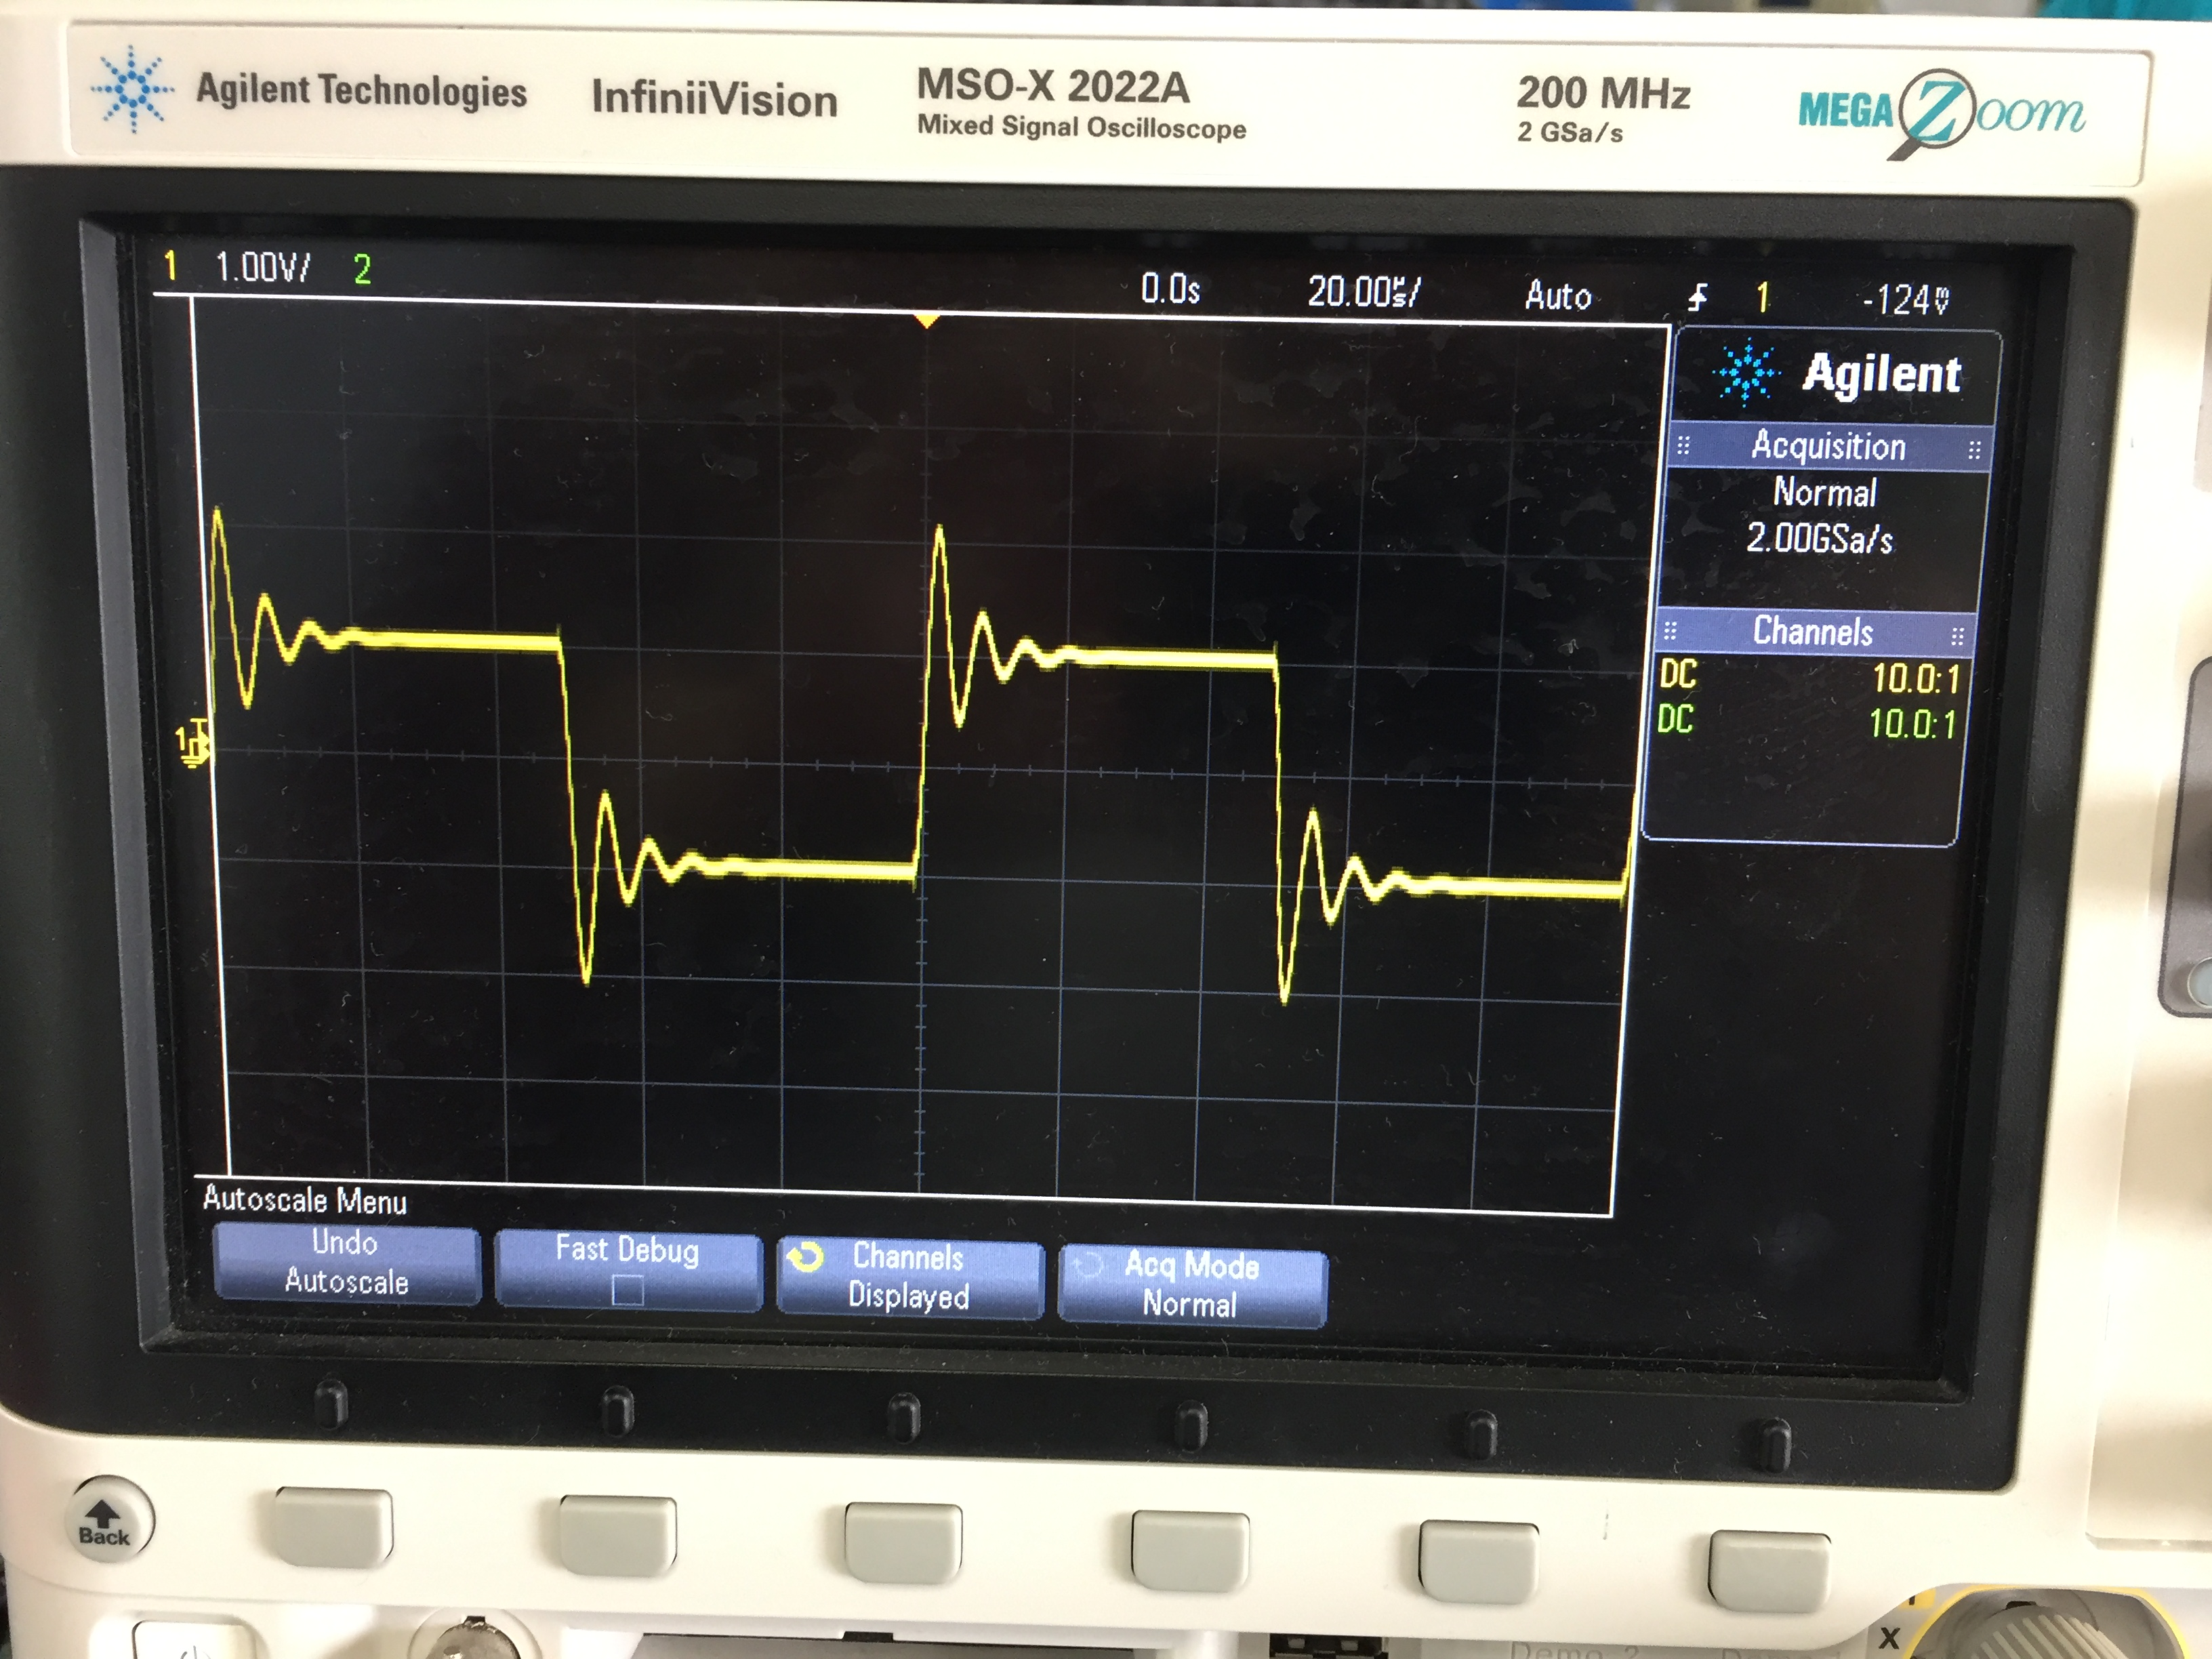
\includegraphics[width=0.7\linewidth]{IMG_6439}
	\label{fig:img6439}
\end{figure}
\begin{figure}[H]
	\centering
	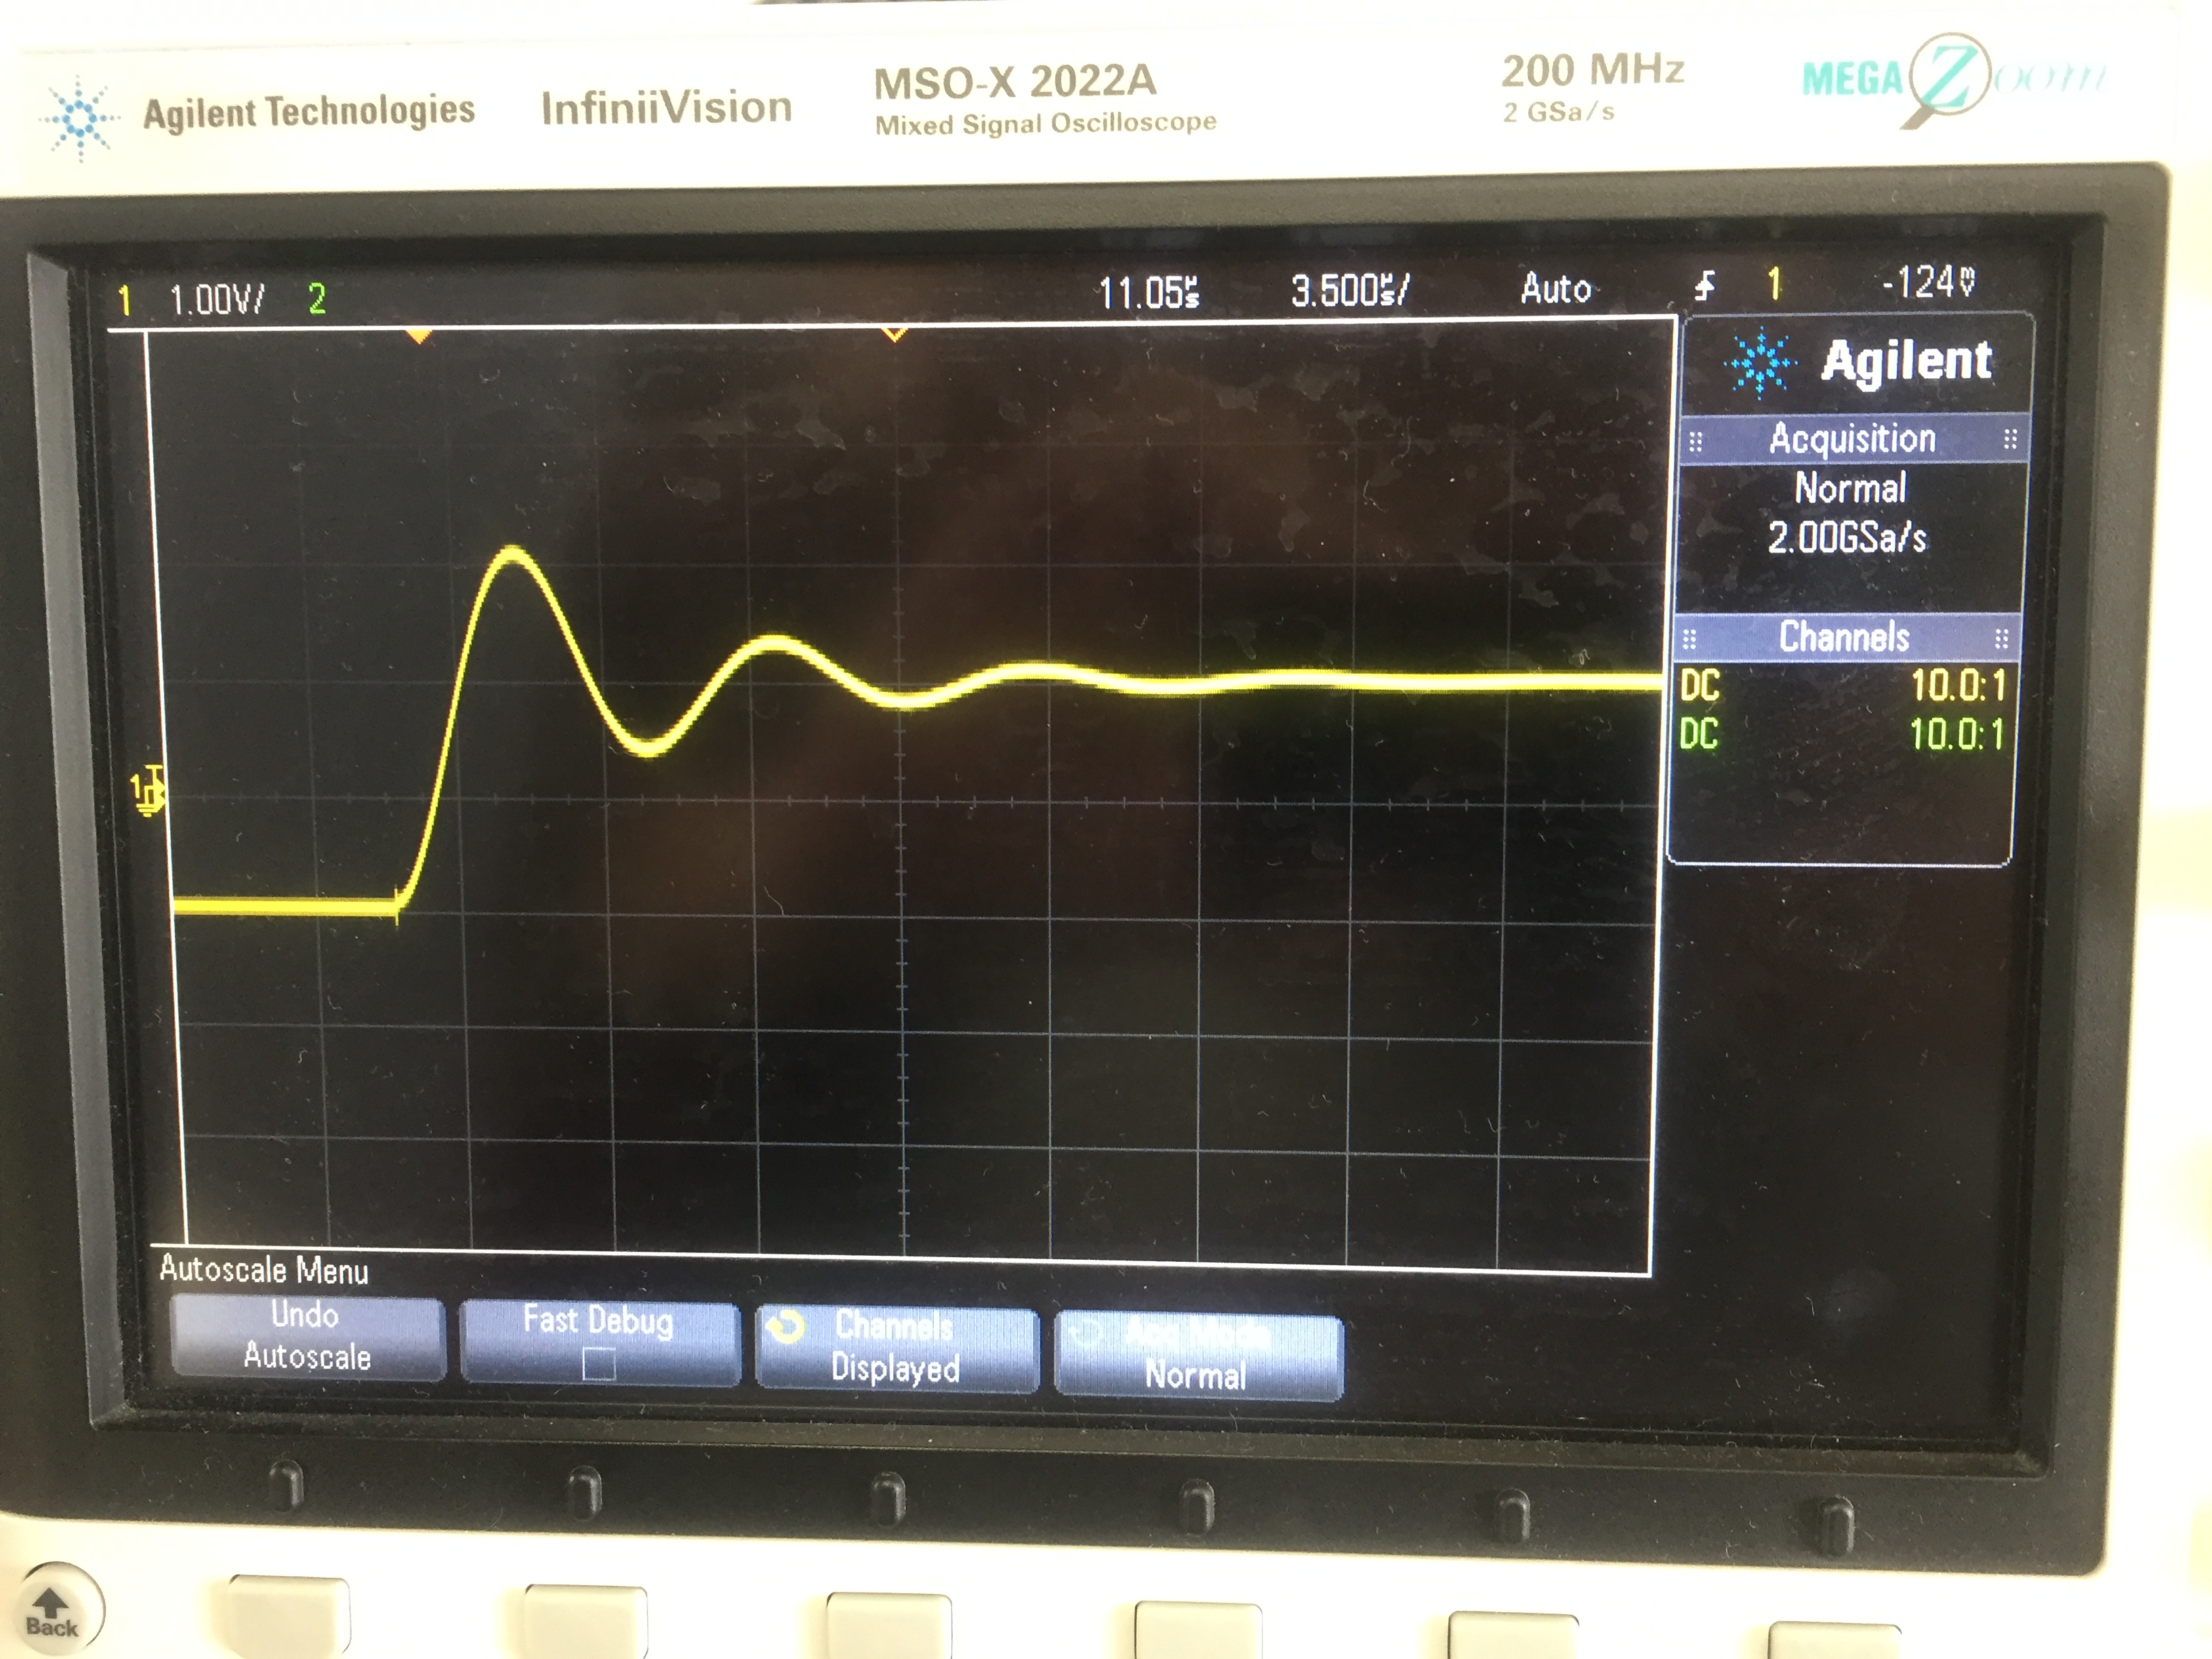
\includegraphics[width=0.7\linewidth]{IMG_6440}
	\label{fig:img6440}
\end{figure}
\begin{figure}[H]
	\centering
	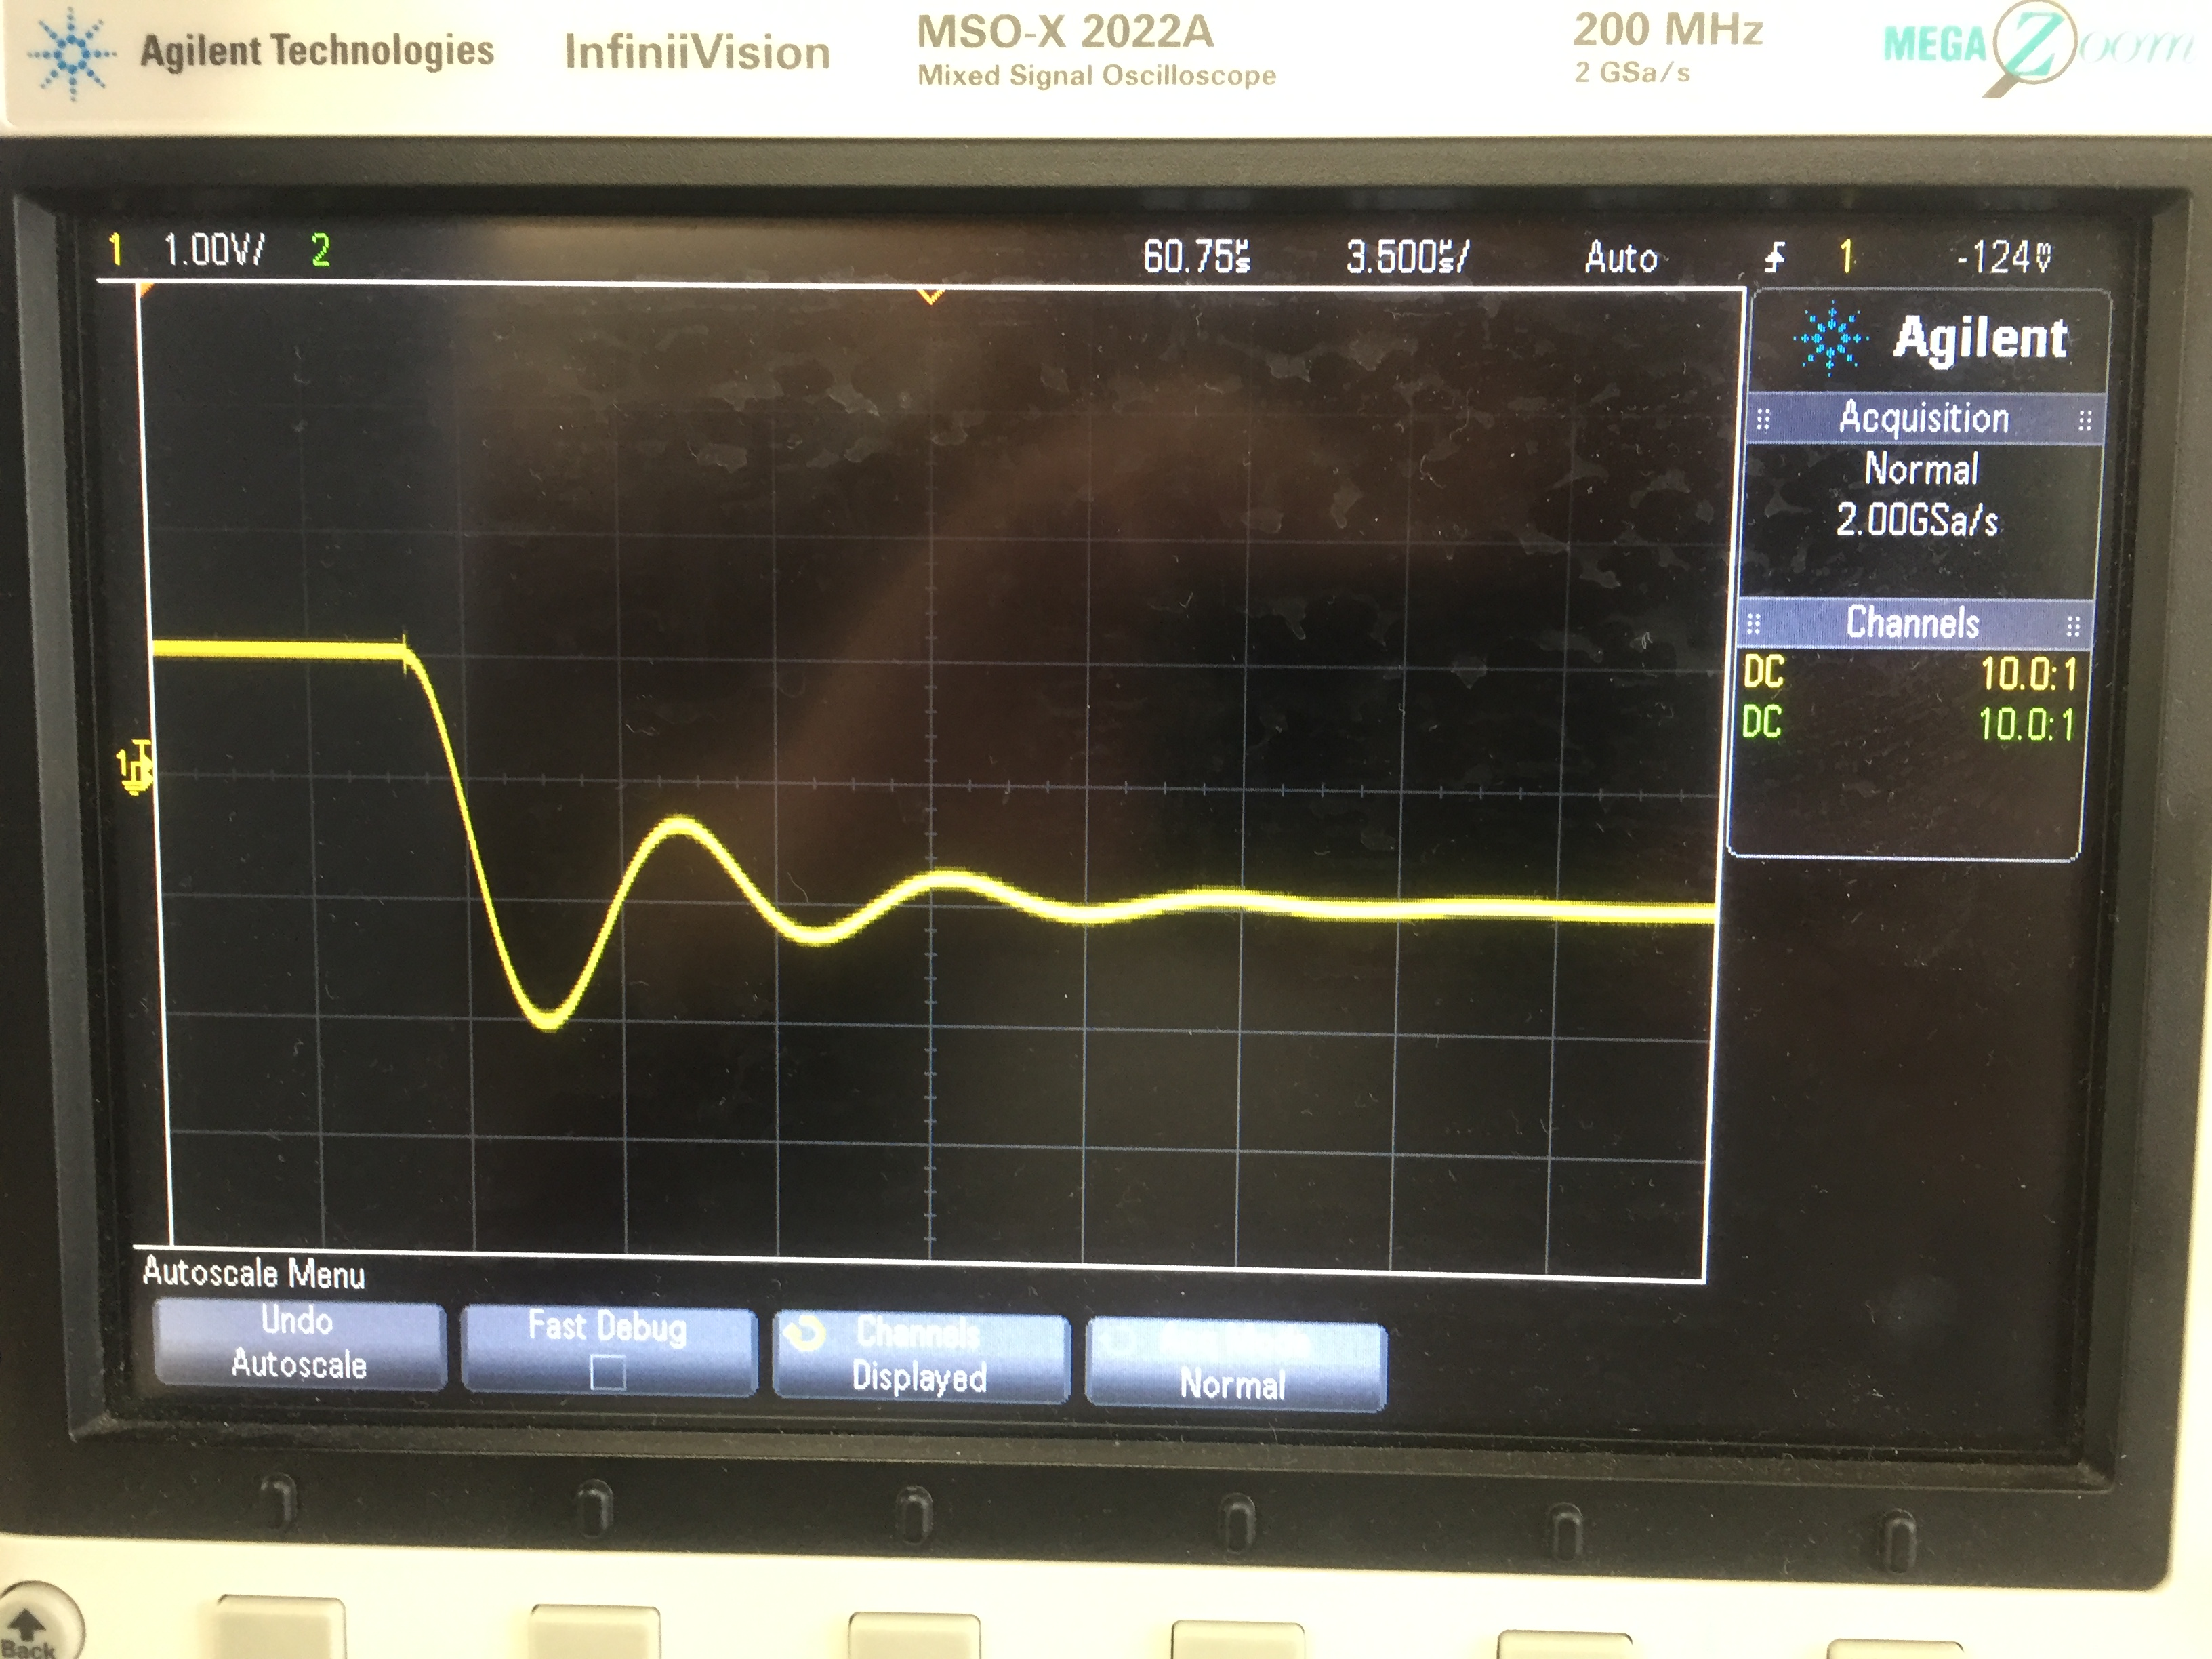
\includegraphics[width=0.7\linewidth]{IMG_6441}
	\label{fig:img6441}
\end{figure}
\begin{figure}[H]
	\centering
	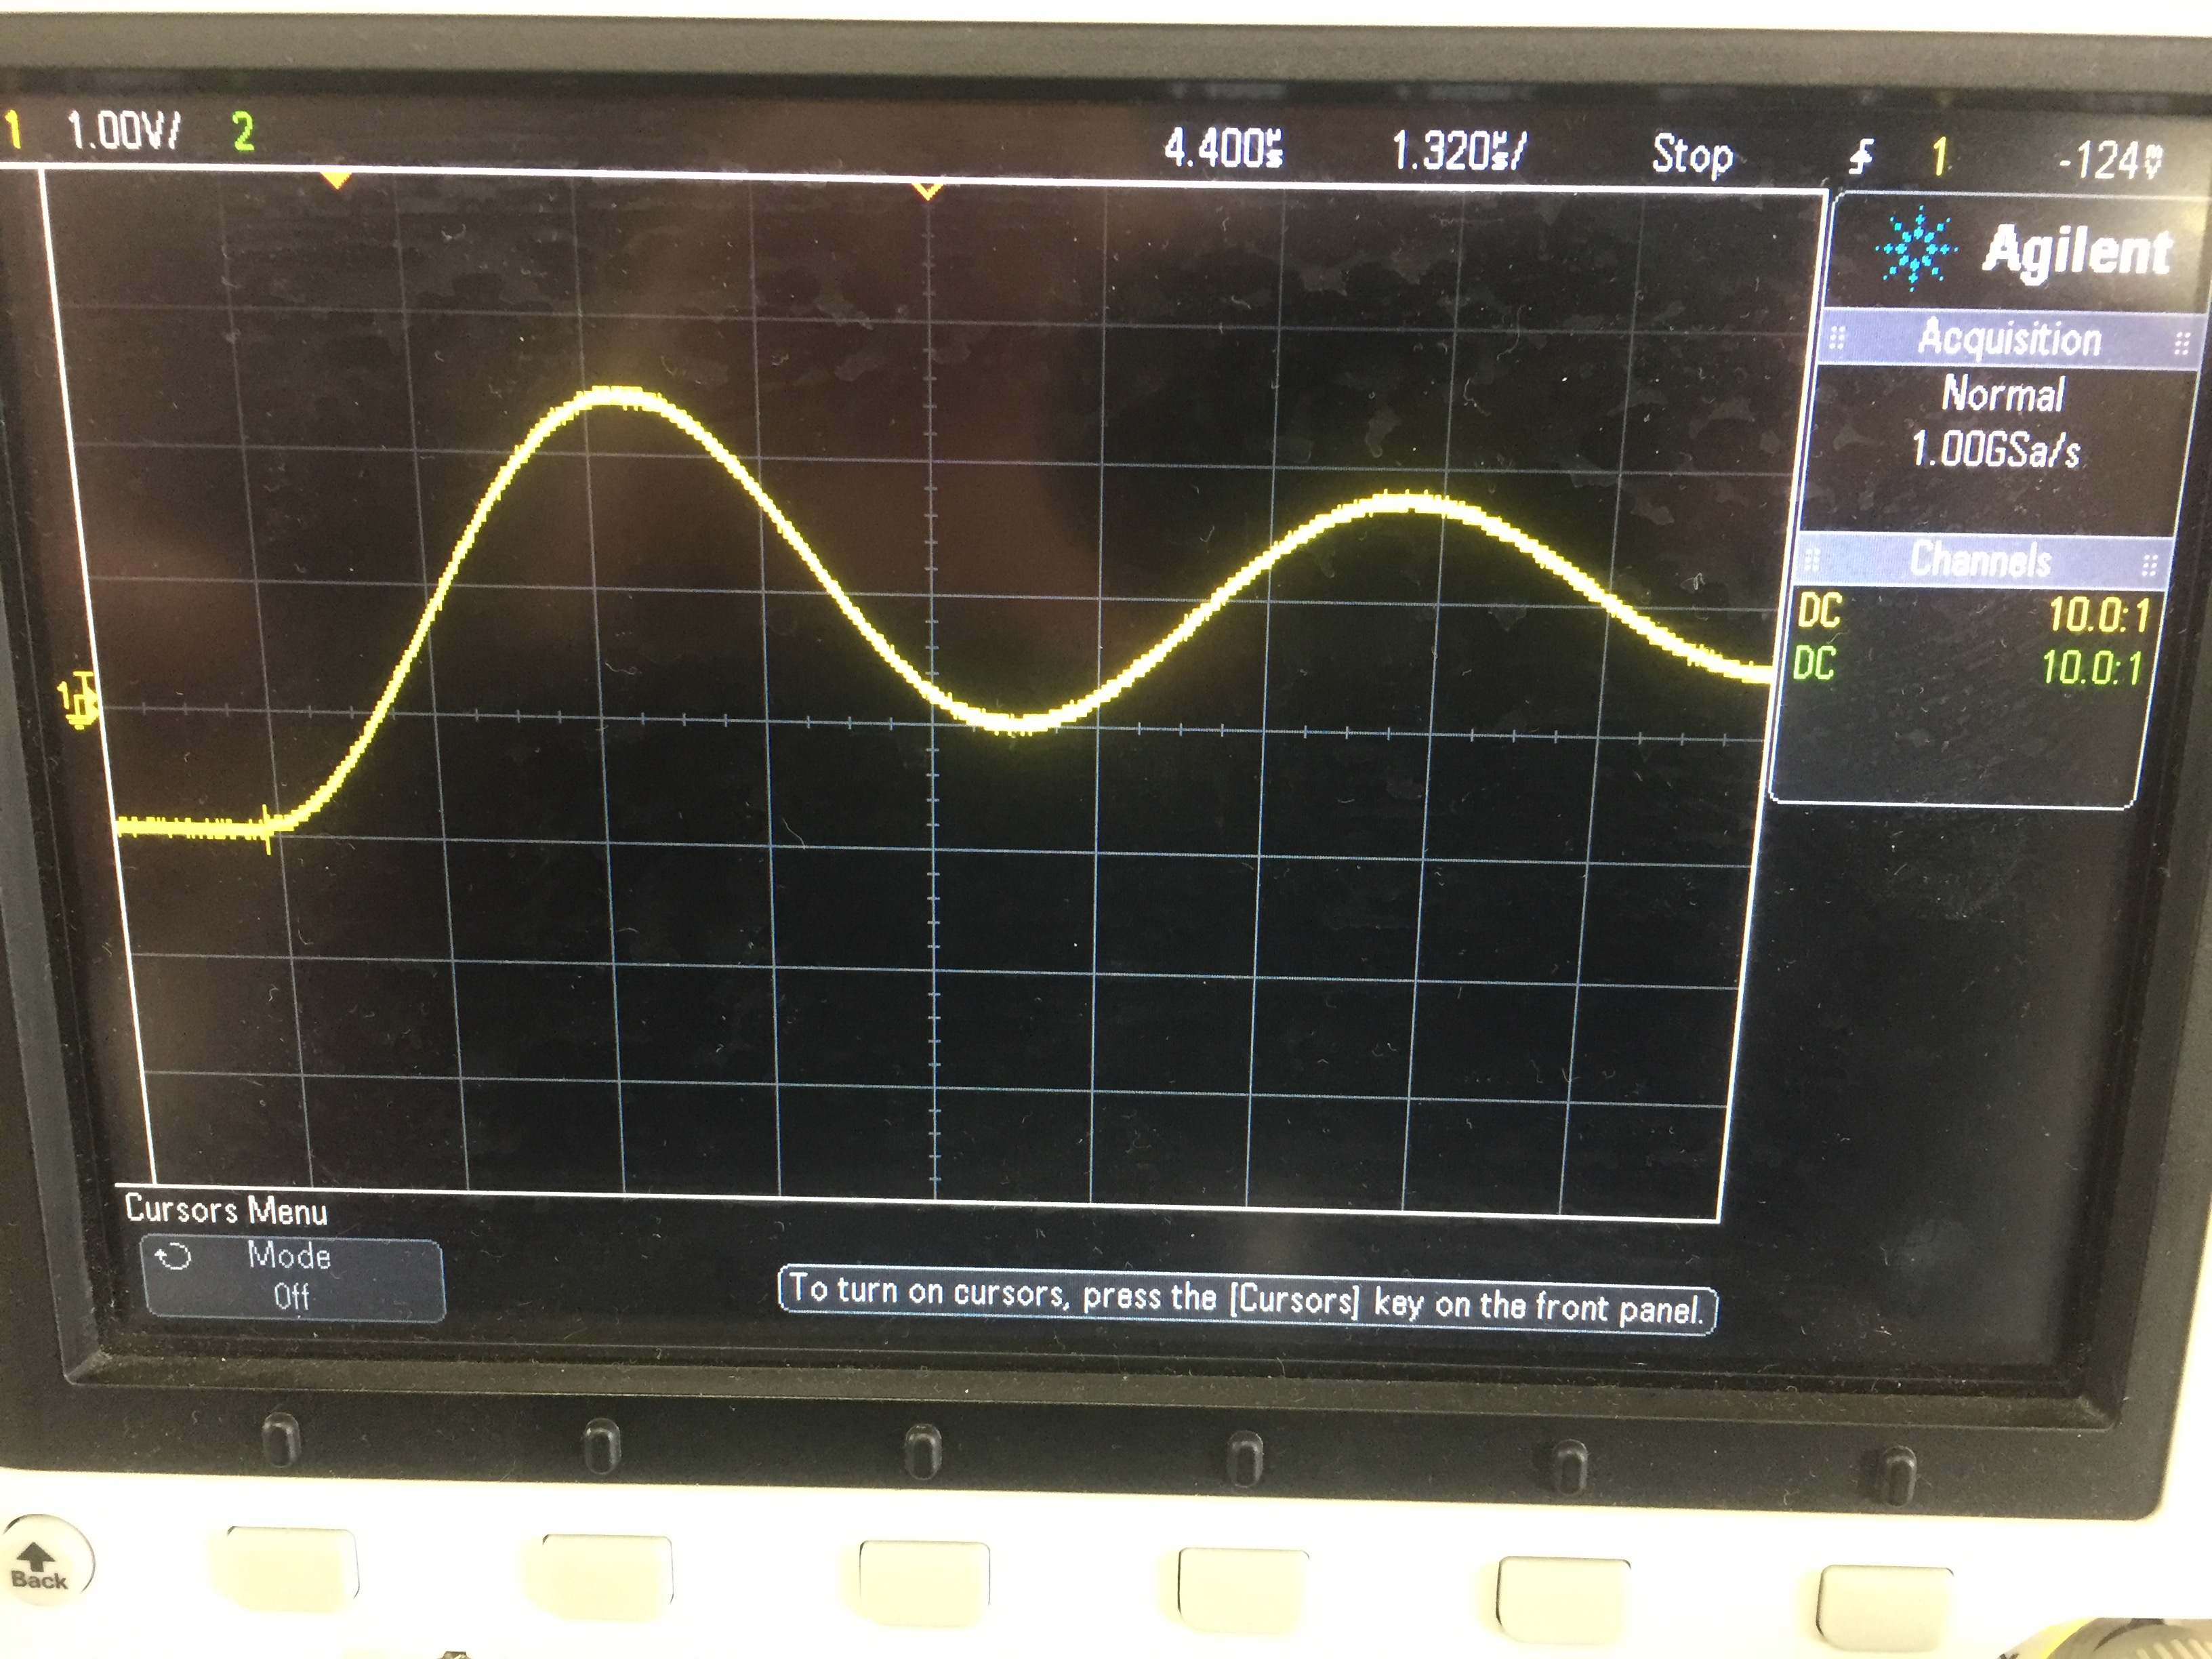
\includegraphics[width=0.7\linewidth]{IMG_6442}
	\label{fig:img6442}
\end{figure}
\begin{figure}[H]
	\centering
	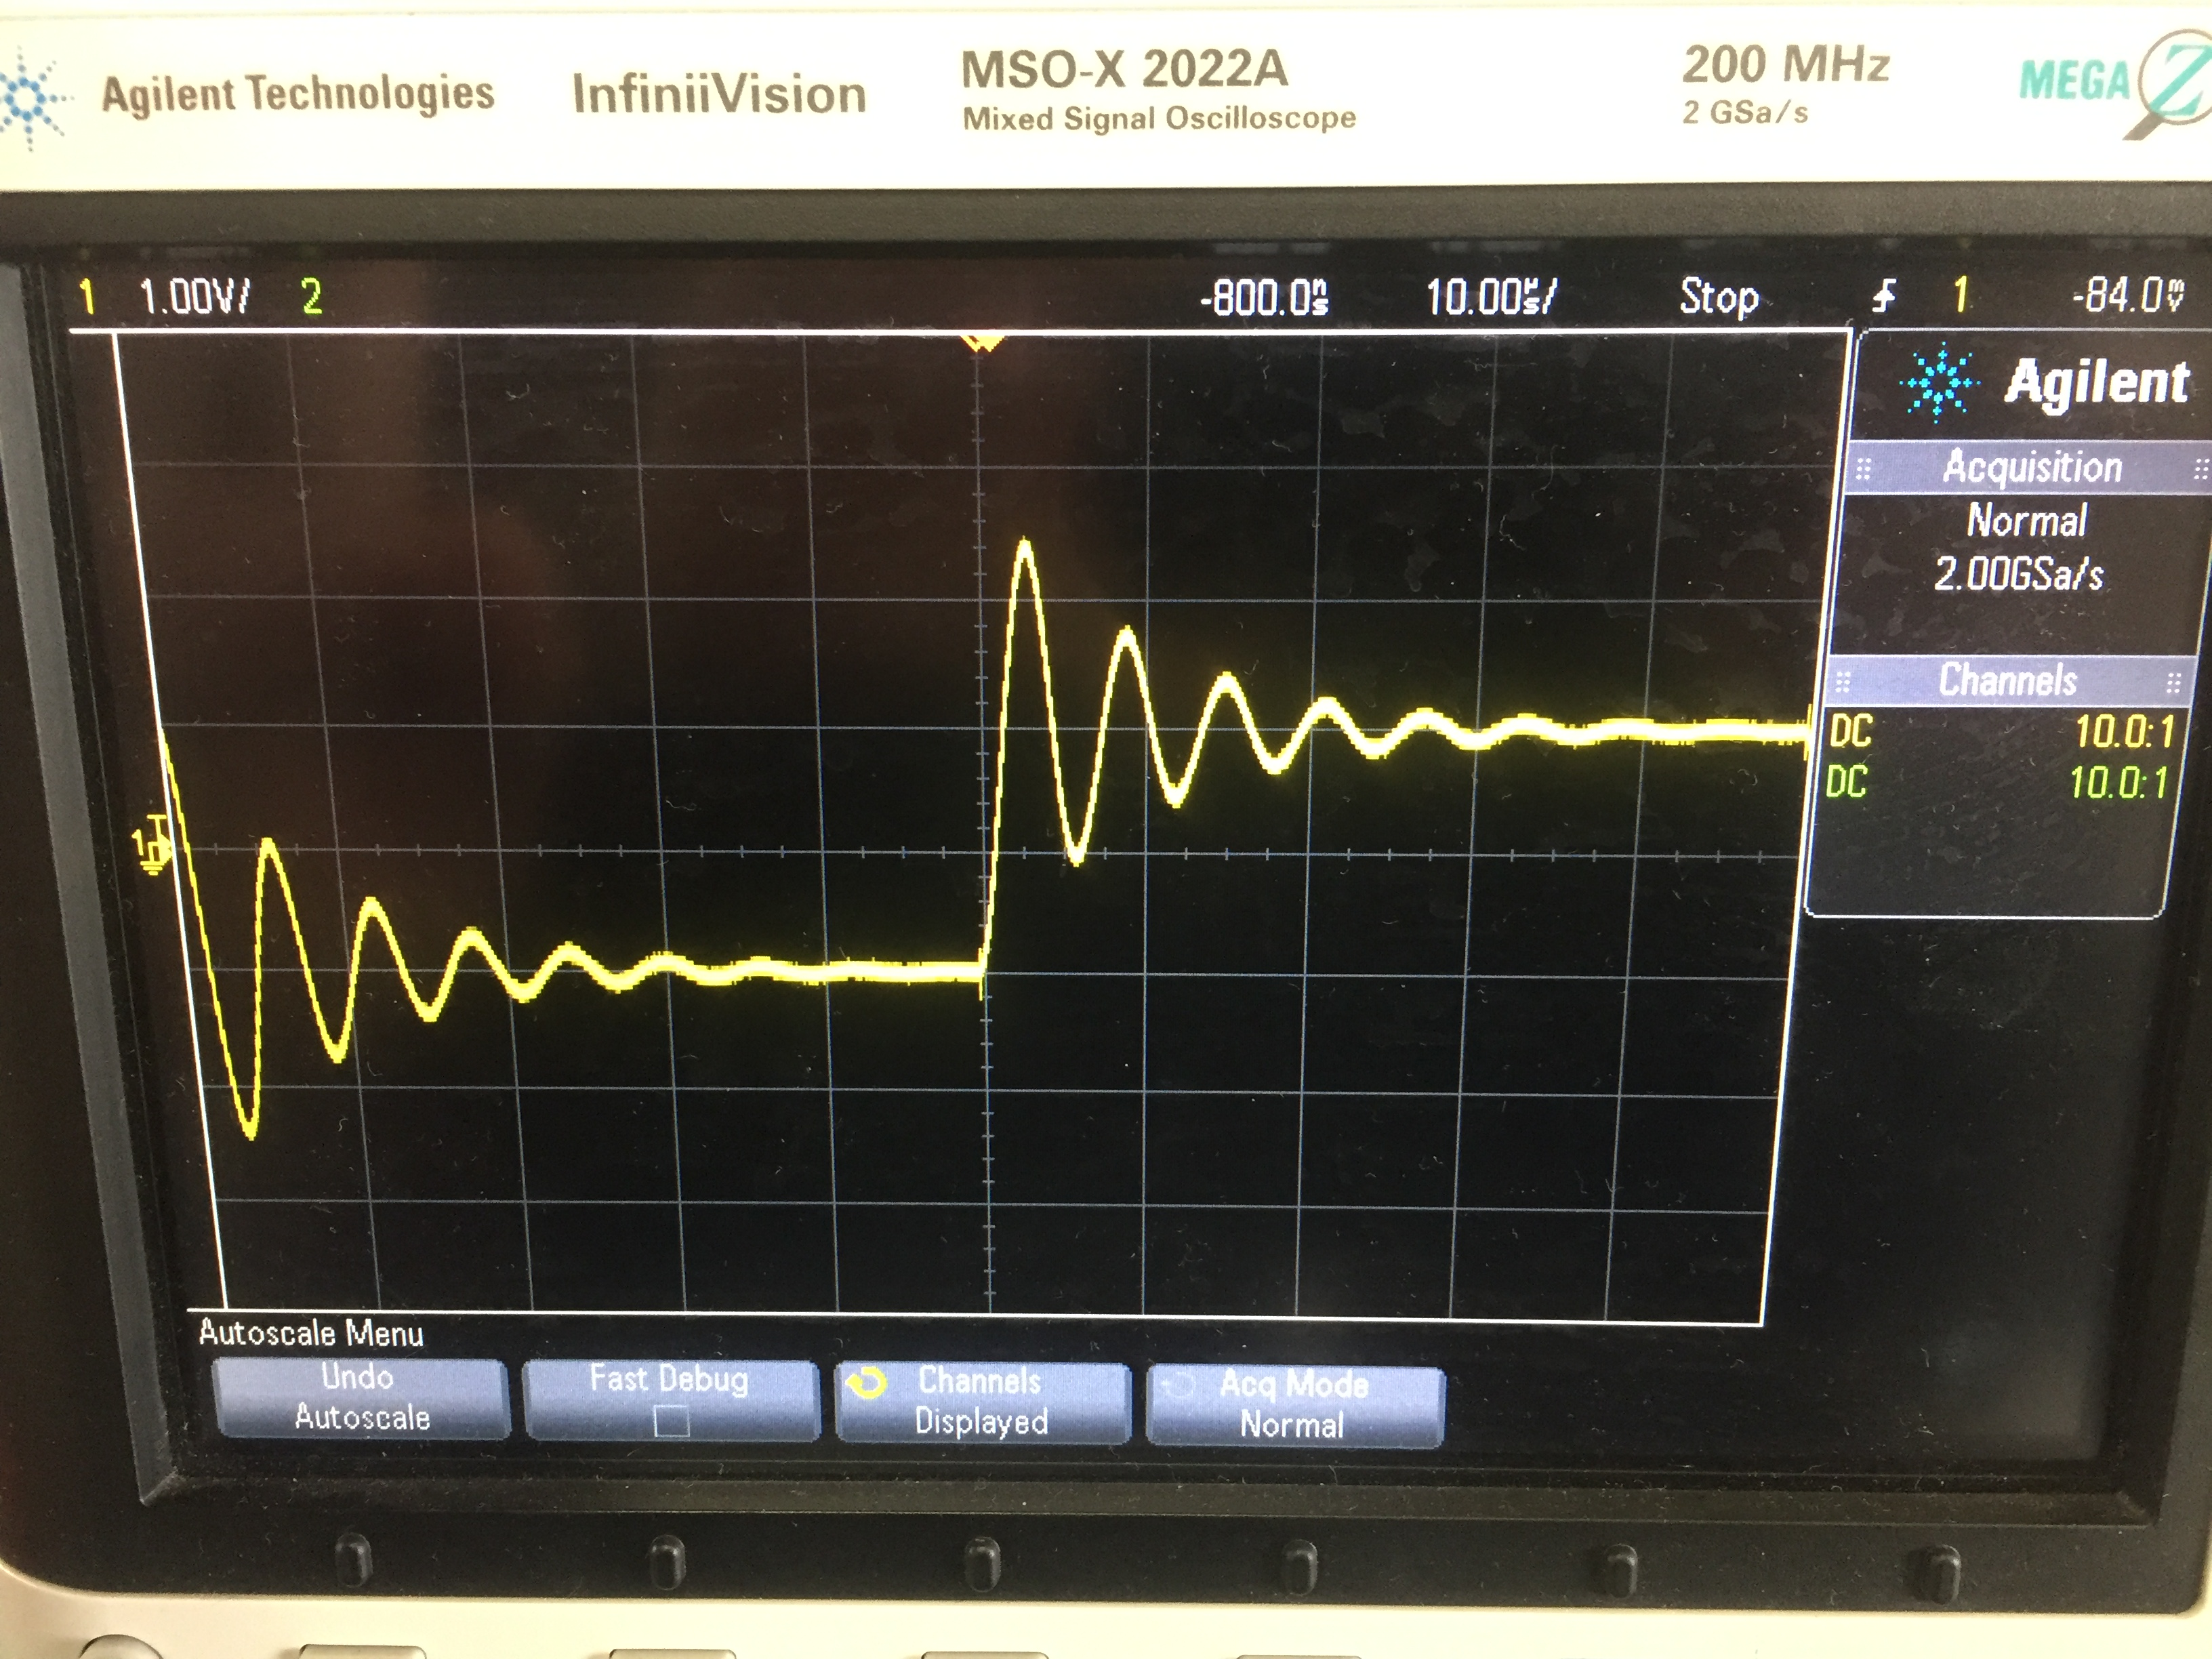
\includegraphics[width=0.7\linewidth]{IMG_6443}
	\label{fig:img6443}
\end{figure}
\begin{figure}[H]
	\centering
	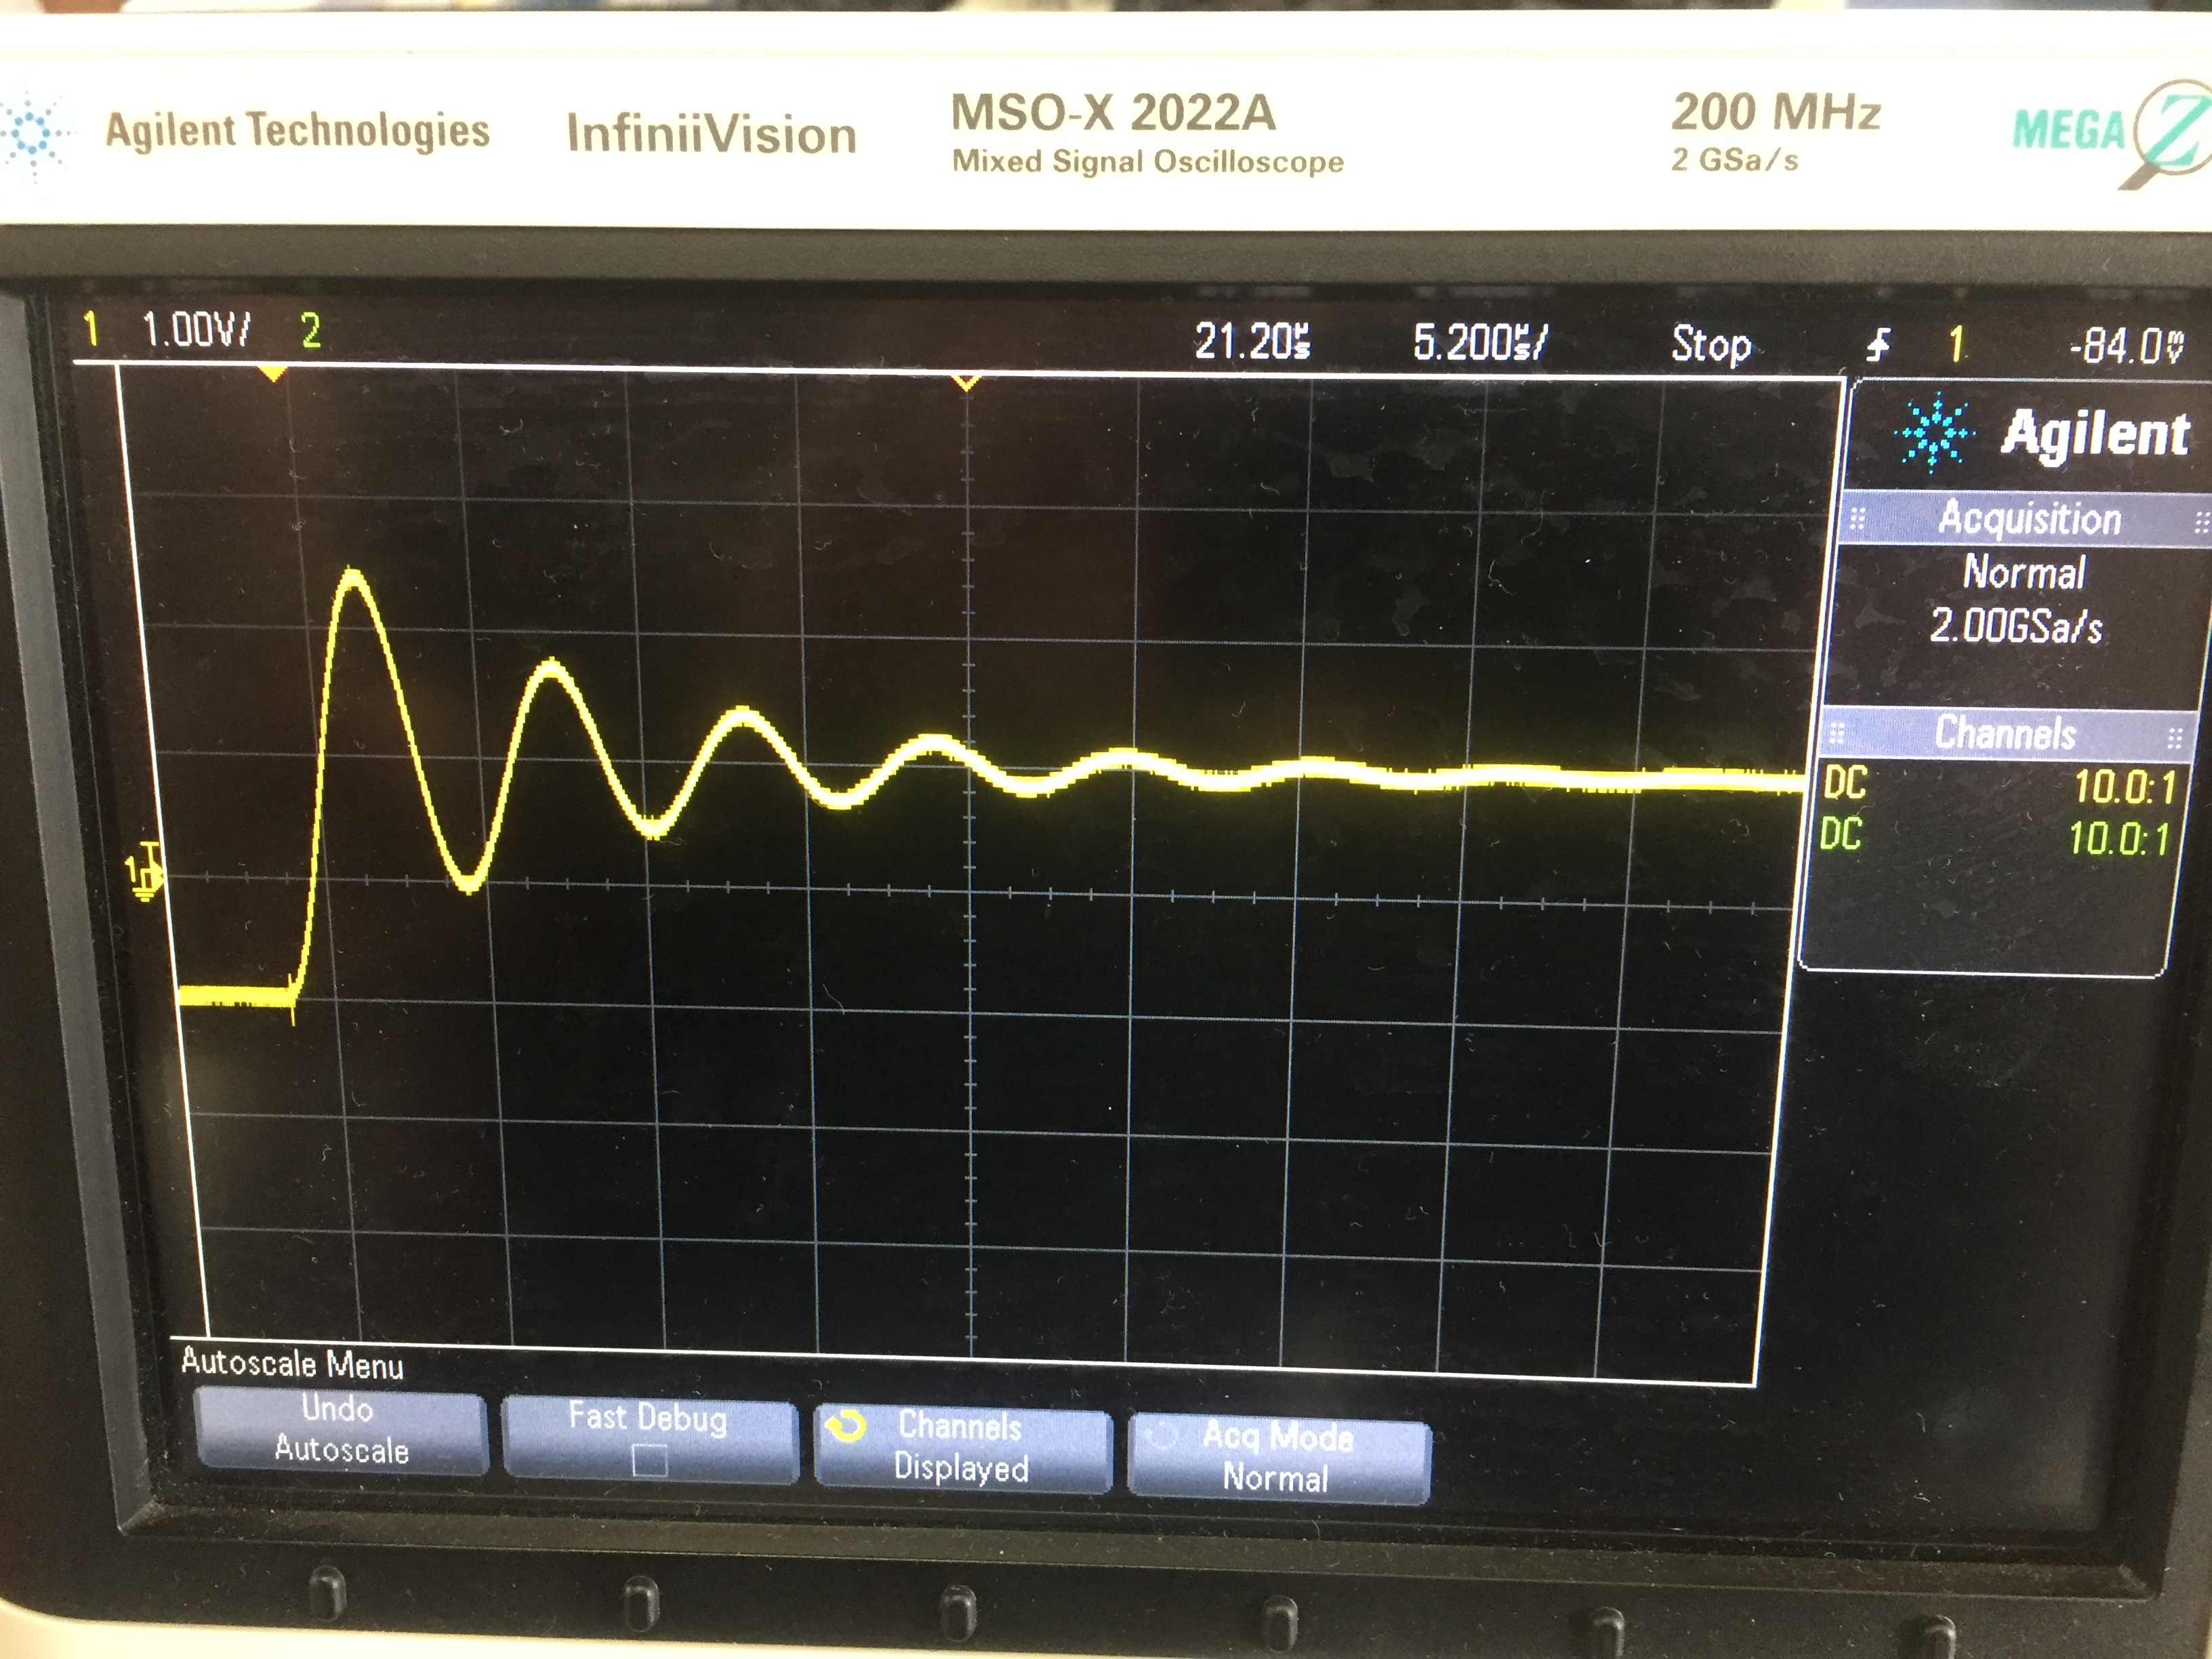
\includegraphics[width=0.7\linewidth]{IMG_6444}
	\label{fig:img6444}
\end{figure}
\begin{figure}[H]
	\centering
	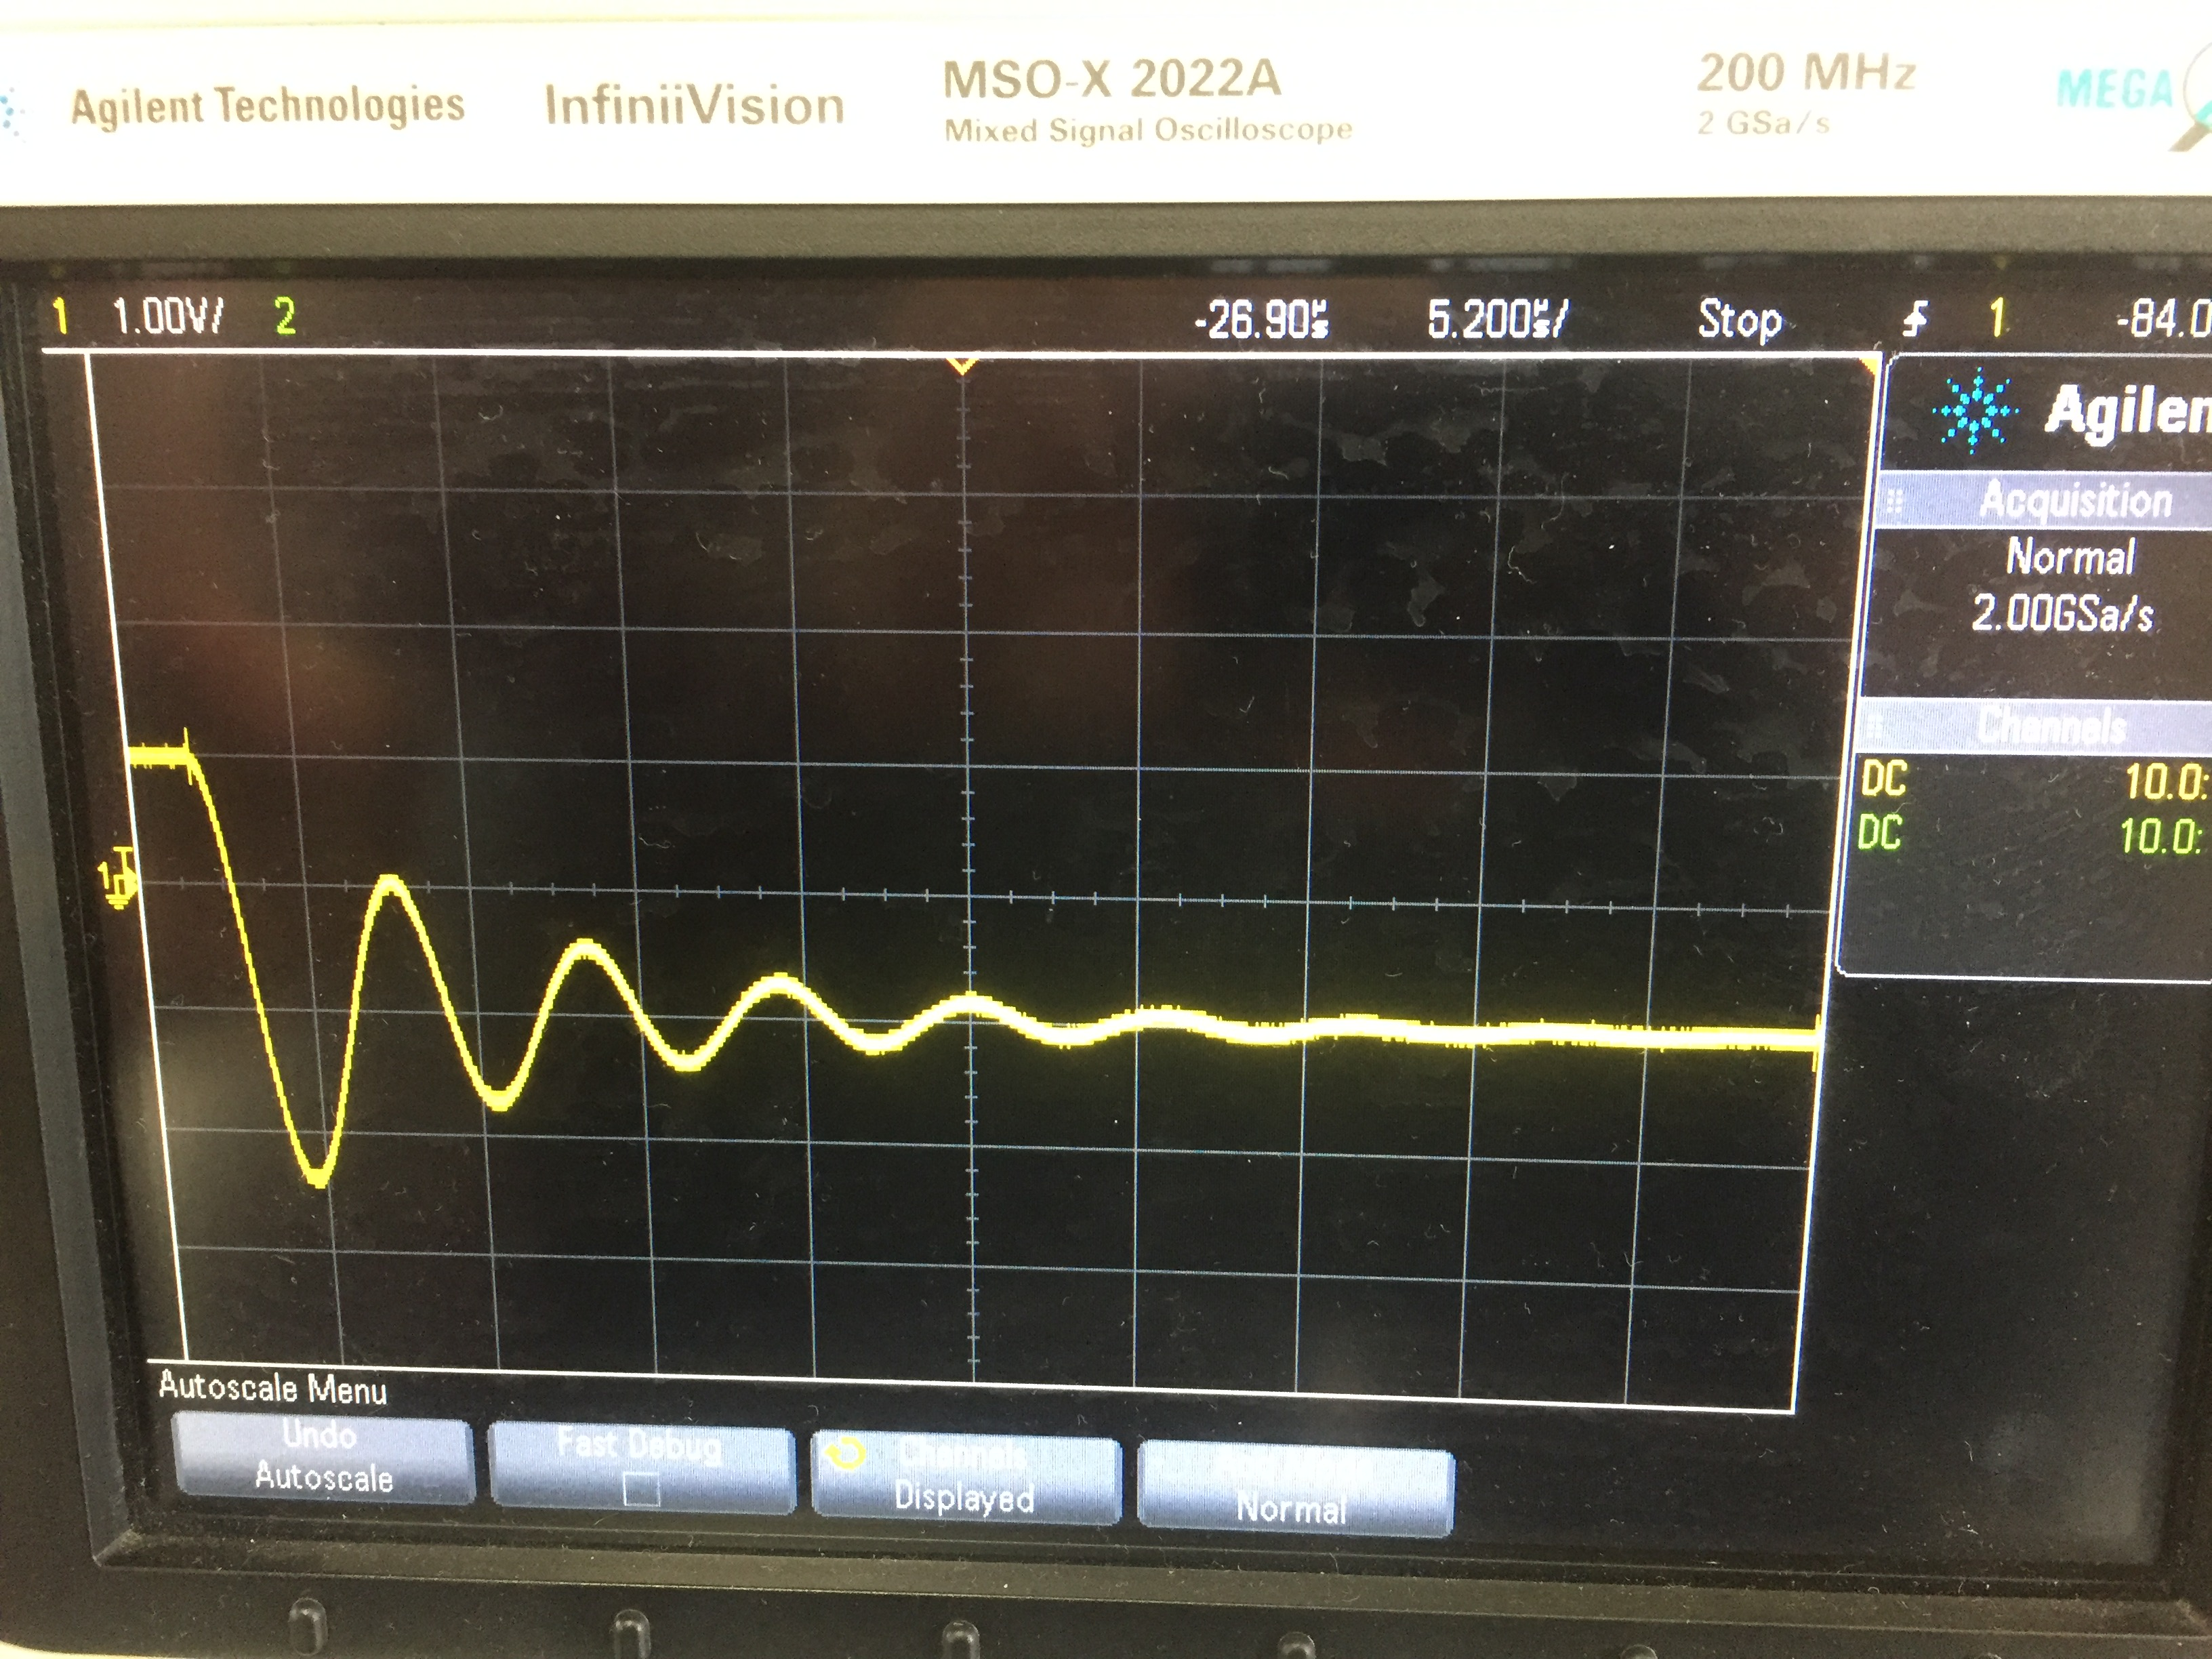
\includegraphics[width=0.7\linewidth]{IMG_6445}
	\label{fig:img6445}
\end{figure}
\begin{figure}[H]
	\centering
	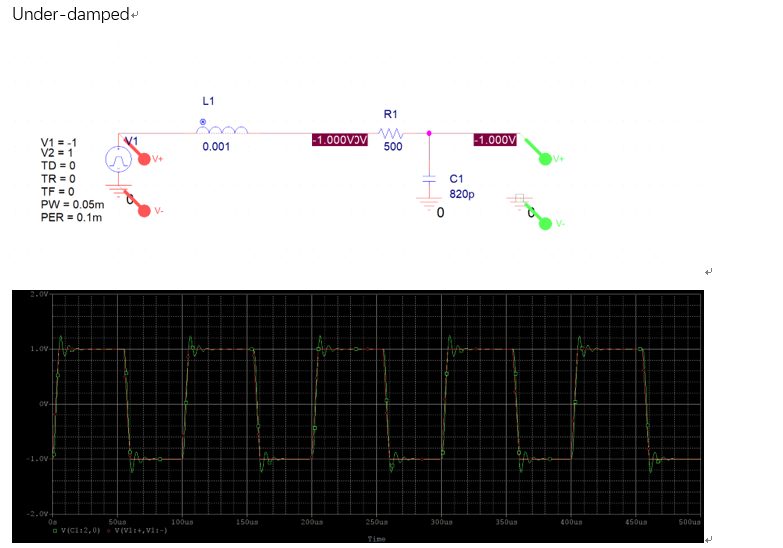
\includegraphics[width=0.7\linewidth]{p1}
	\caption{Under-damped}
	\label{fig:p1}
\end{figure}
From the simulation by using Pspice, we find that our output is relatively correct.
\begin{figure}[H]
	\centering
	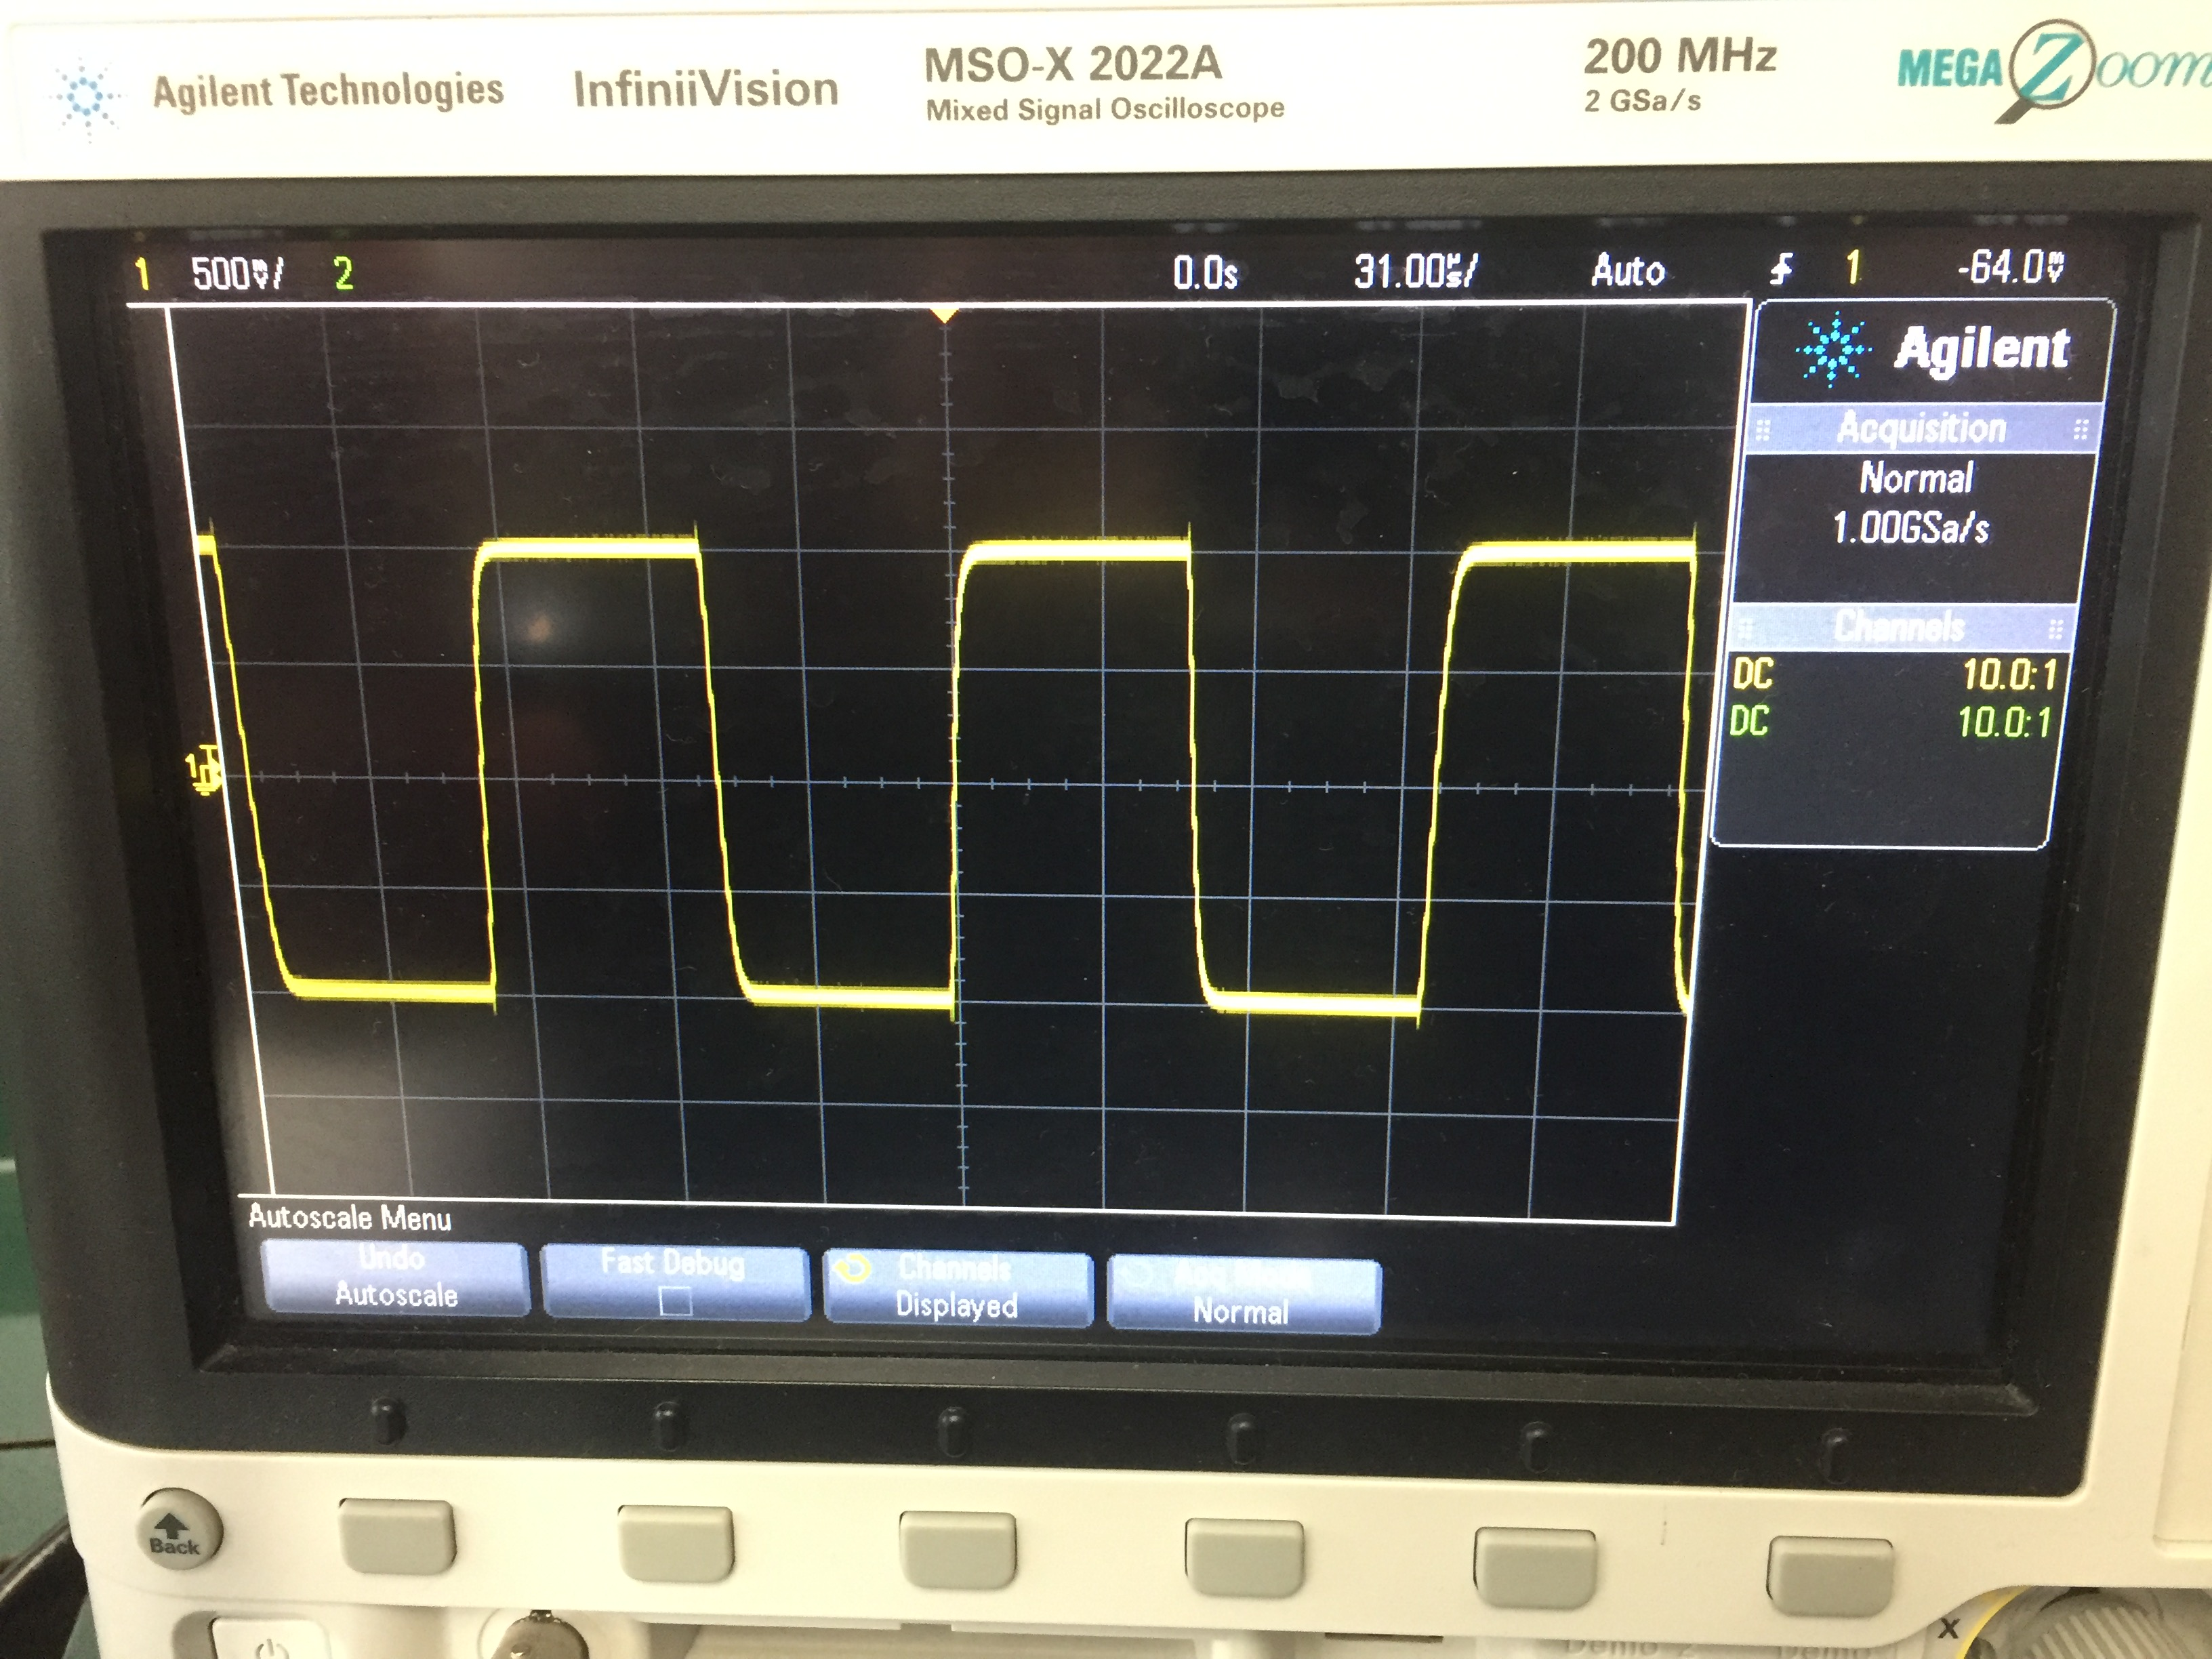
\includegraphics[width=0.7\linewidth]{IMG_6446}
	\label{fig:img6446}
\end{figure}
\begin{figure}[H]
	\centering
	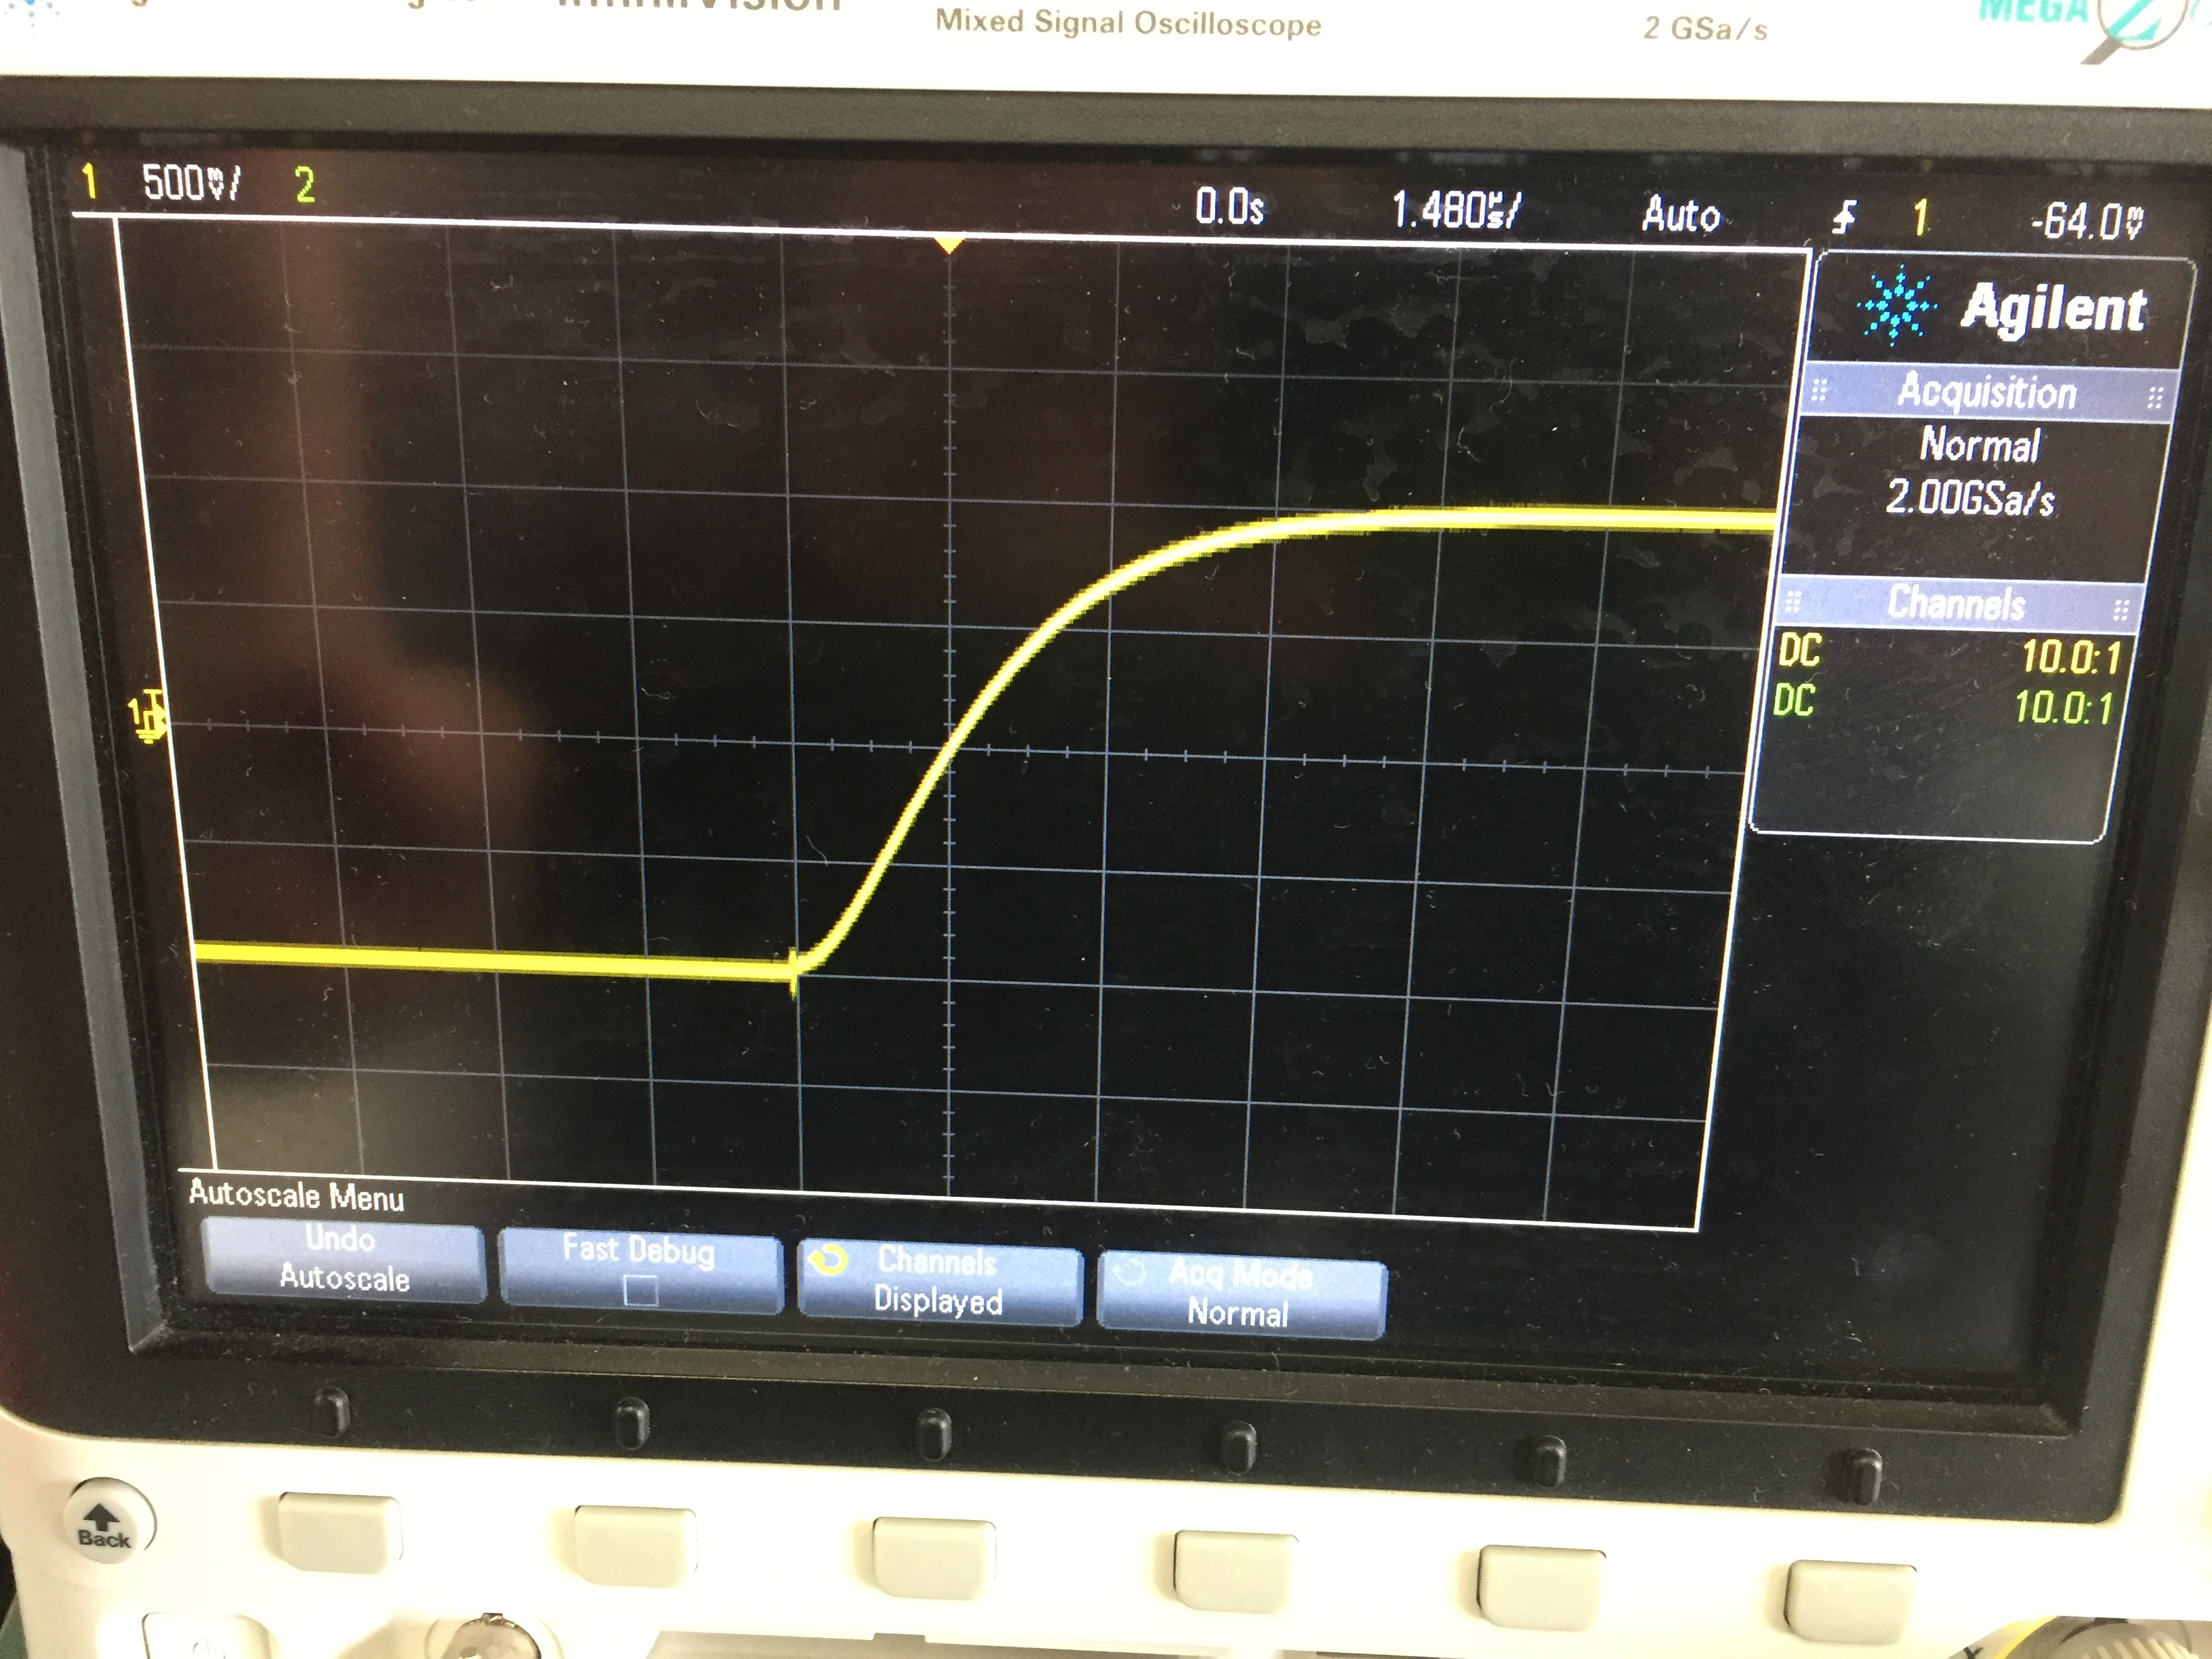
\includegraphics[width=0.7\linewidth]{IMG_6447}
	\label{fig:img6447}
\end{figure}
\begin{figure}[H]
	\centering
	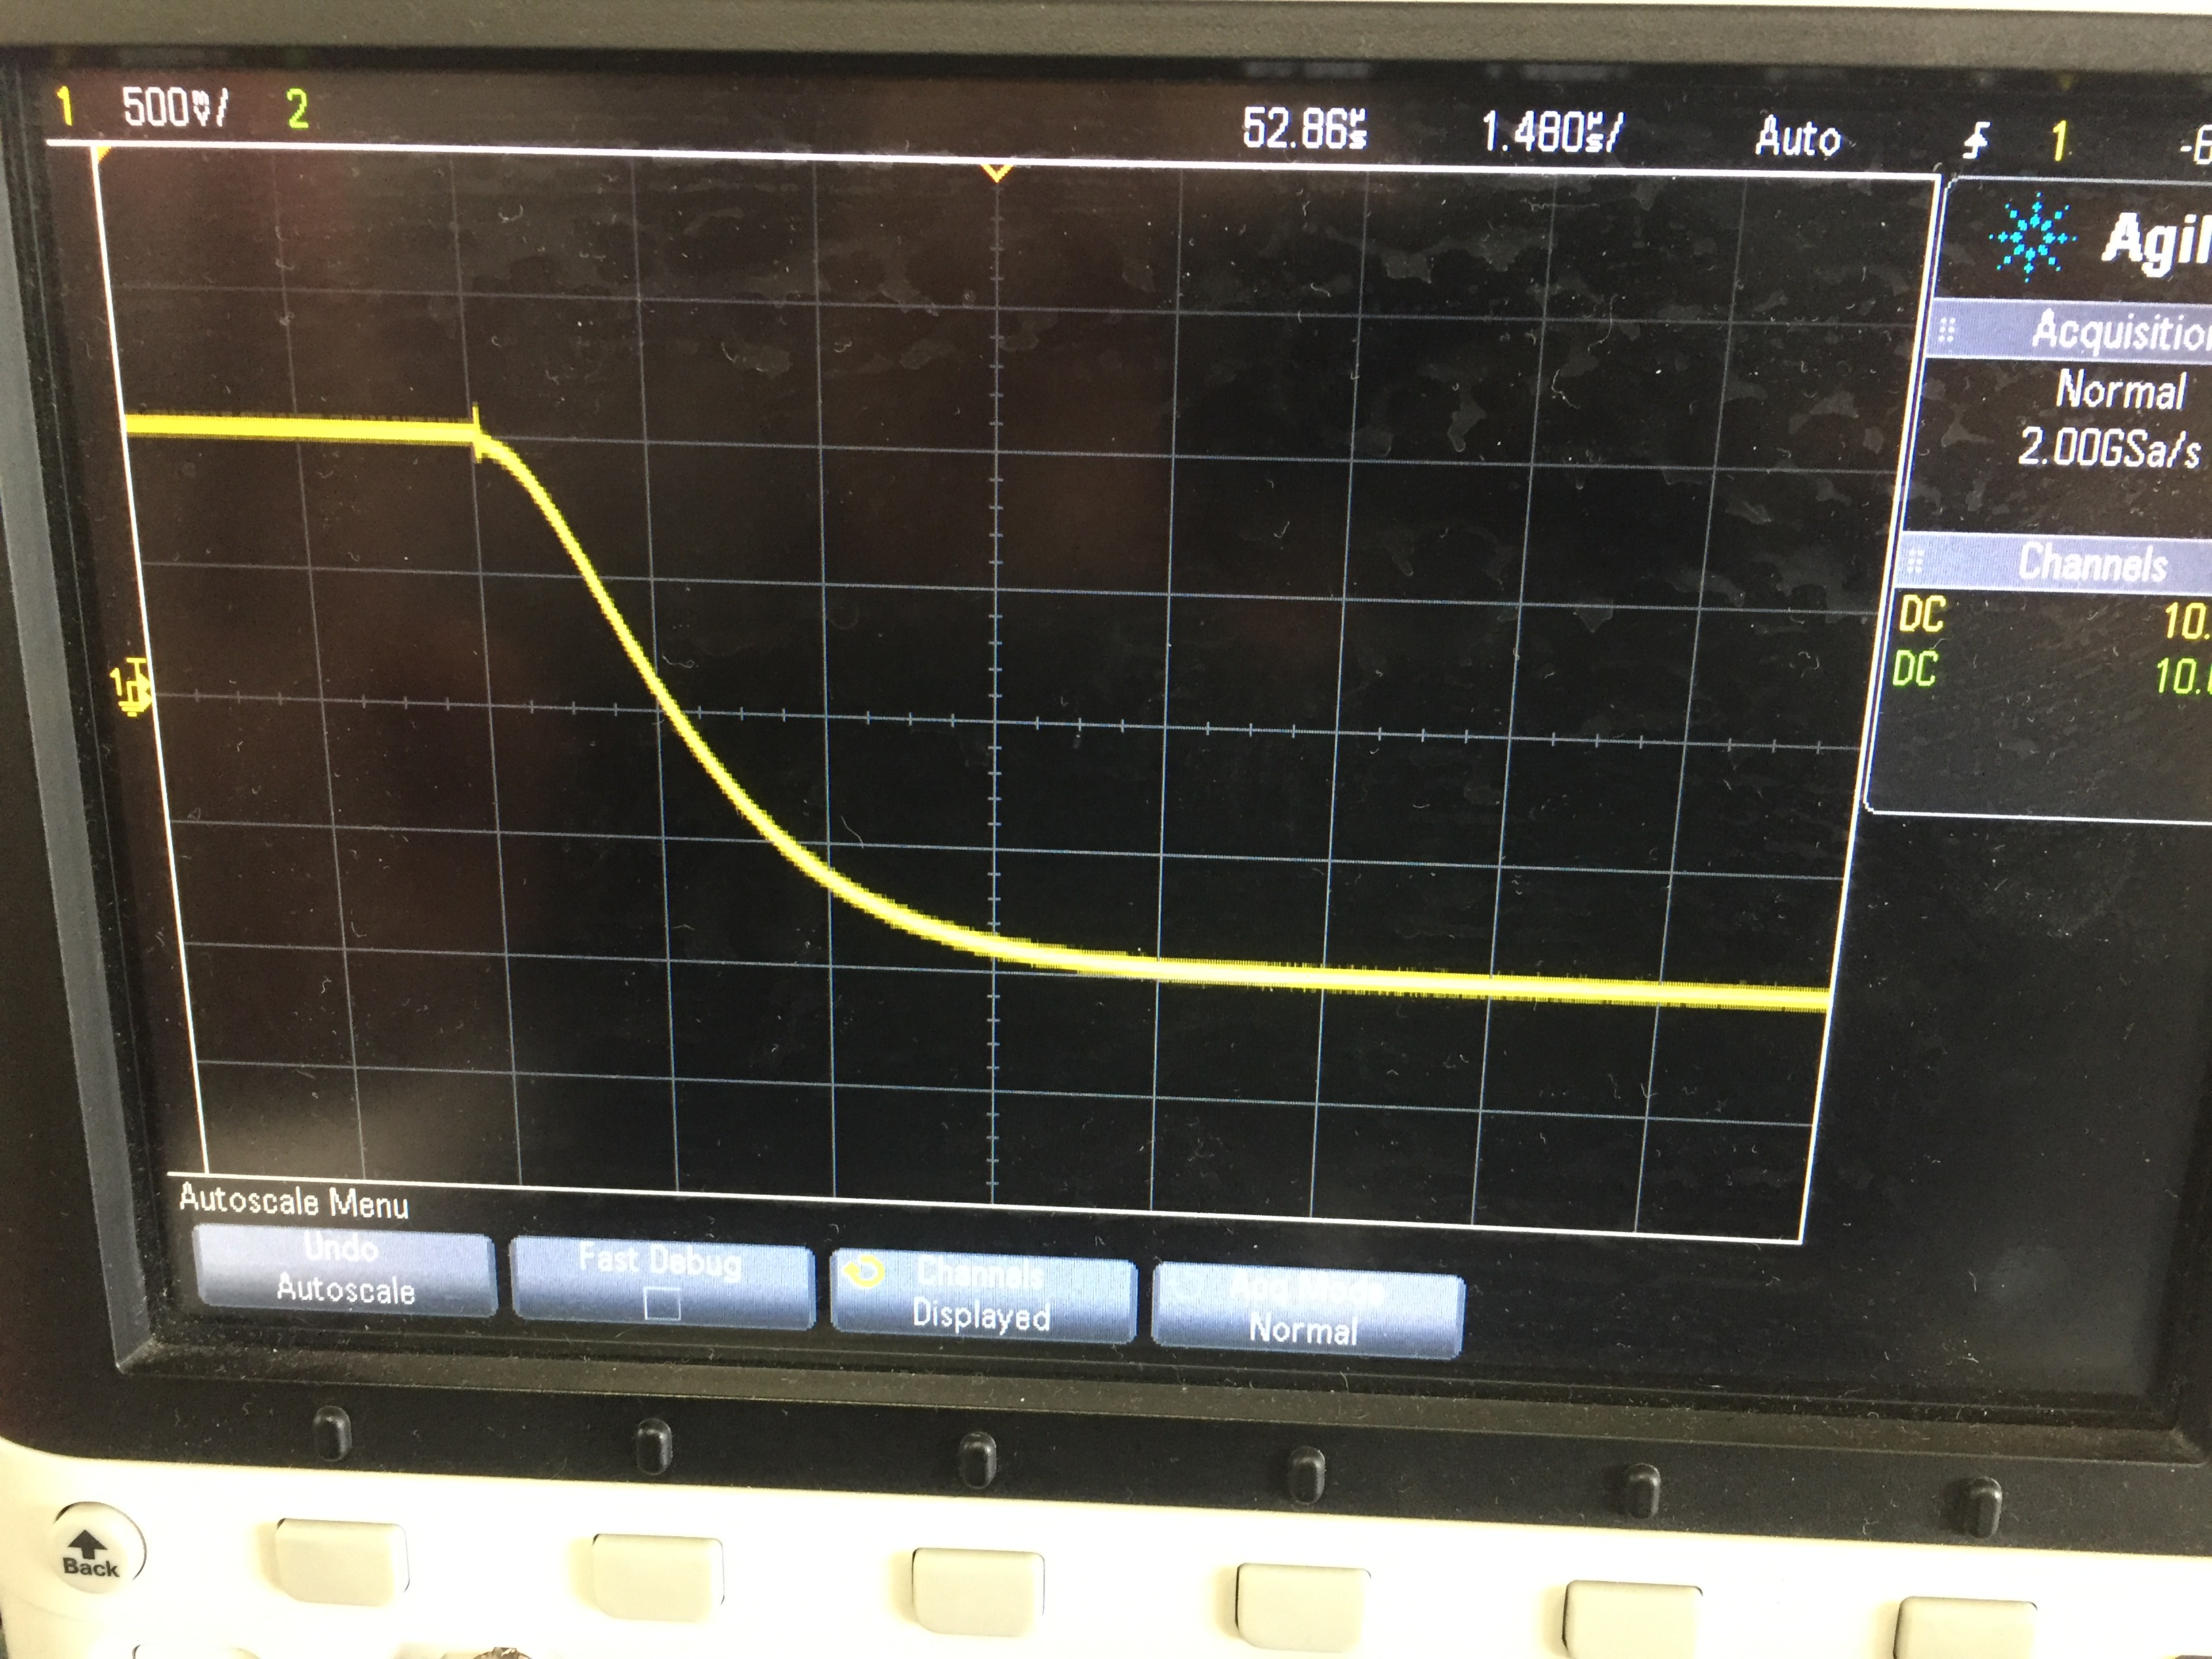
\includegraphics[width=0.7\linewidth]{IMG_6448}
	\label{fig:img6448}
\end{figure}
\begin{figure}[H]
	\centering
	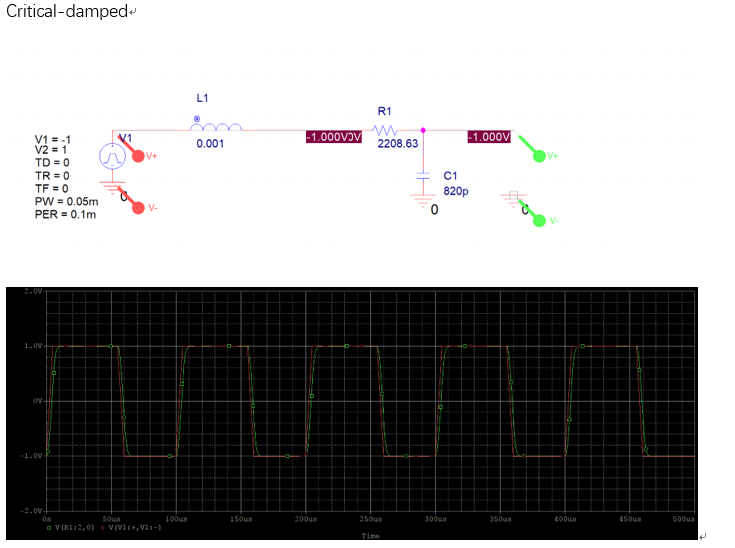
\includegraphics[width=0.7\linewidth]{p2}
	\caption{Critical damped}
	\label{fig:p2}
\end{figure}
From the simulation by using Pspice, we find that our output is relatively correct.
\begin{figure}[H]
	\centering
	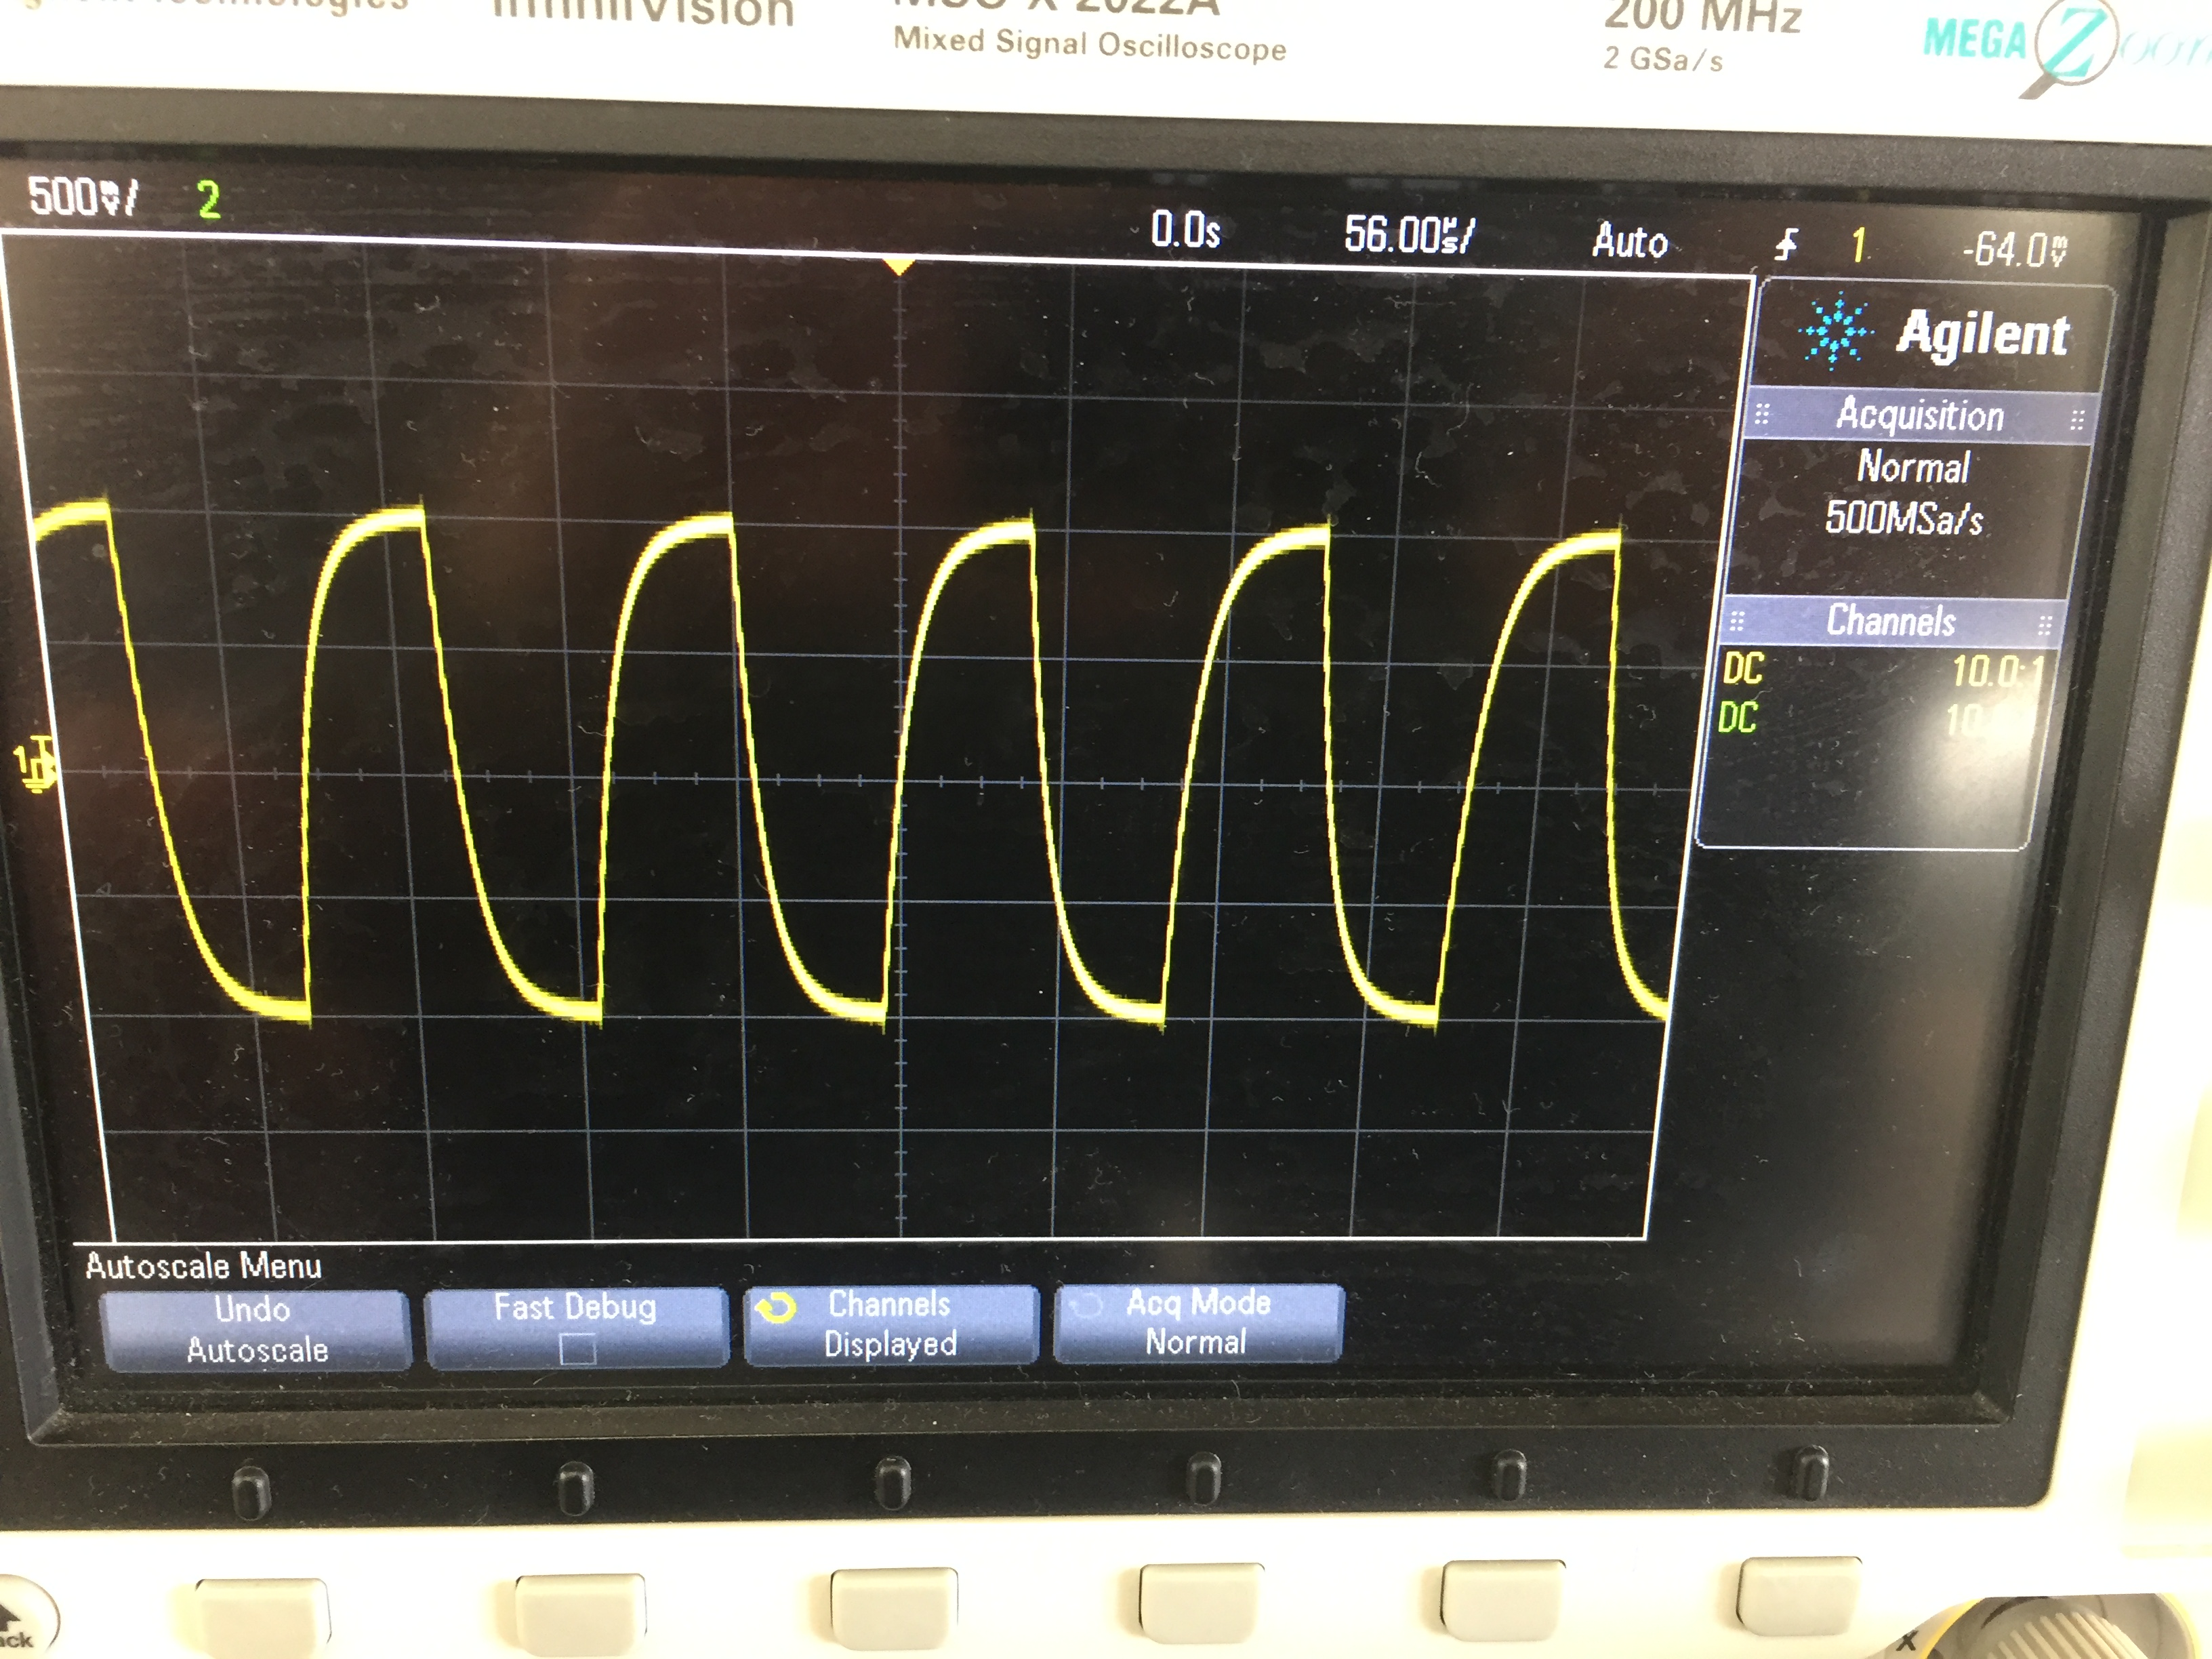
\includegraphics[width=0.7\linewidth]{IMG_6449}
	\label{fig:img6449}
\end{figure}
\begin{figure}[H]
	\centering
	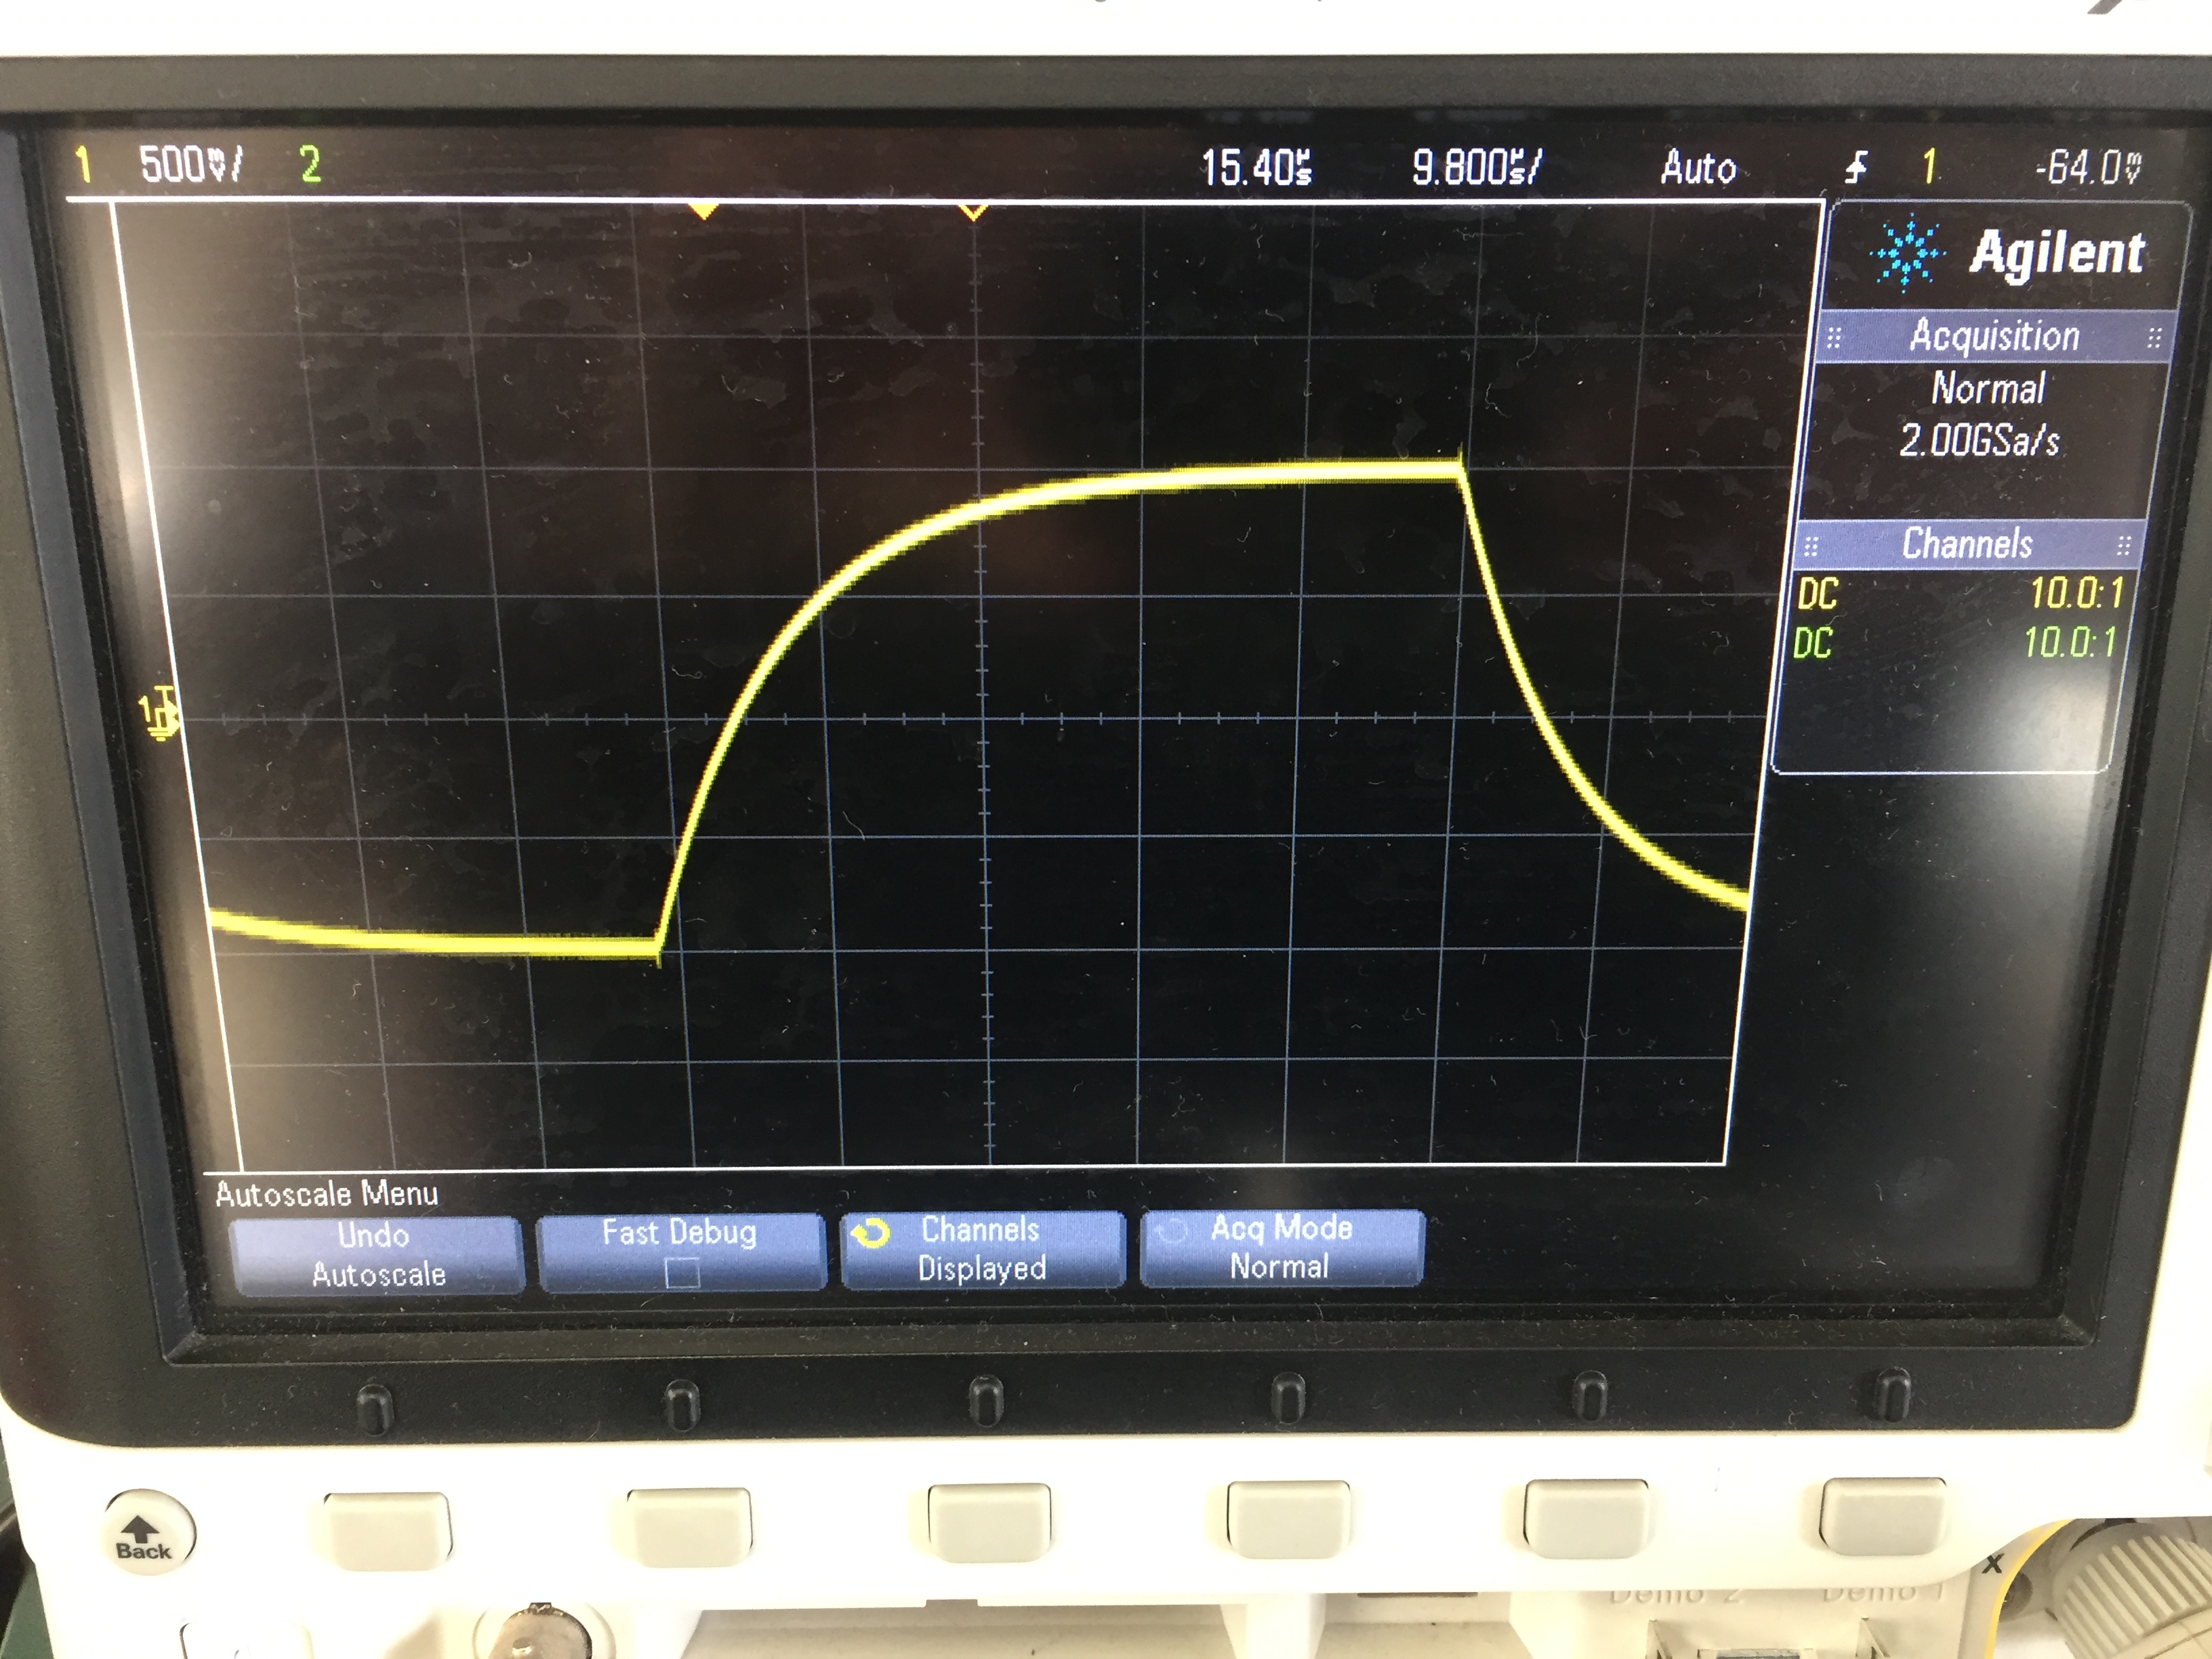
\includegraphics[width=0.7\linewidth]{IMG_6450}
	\label{fig:img6450}
\end{figure}
\begin{figure}[H]
	\centering
	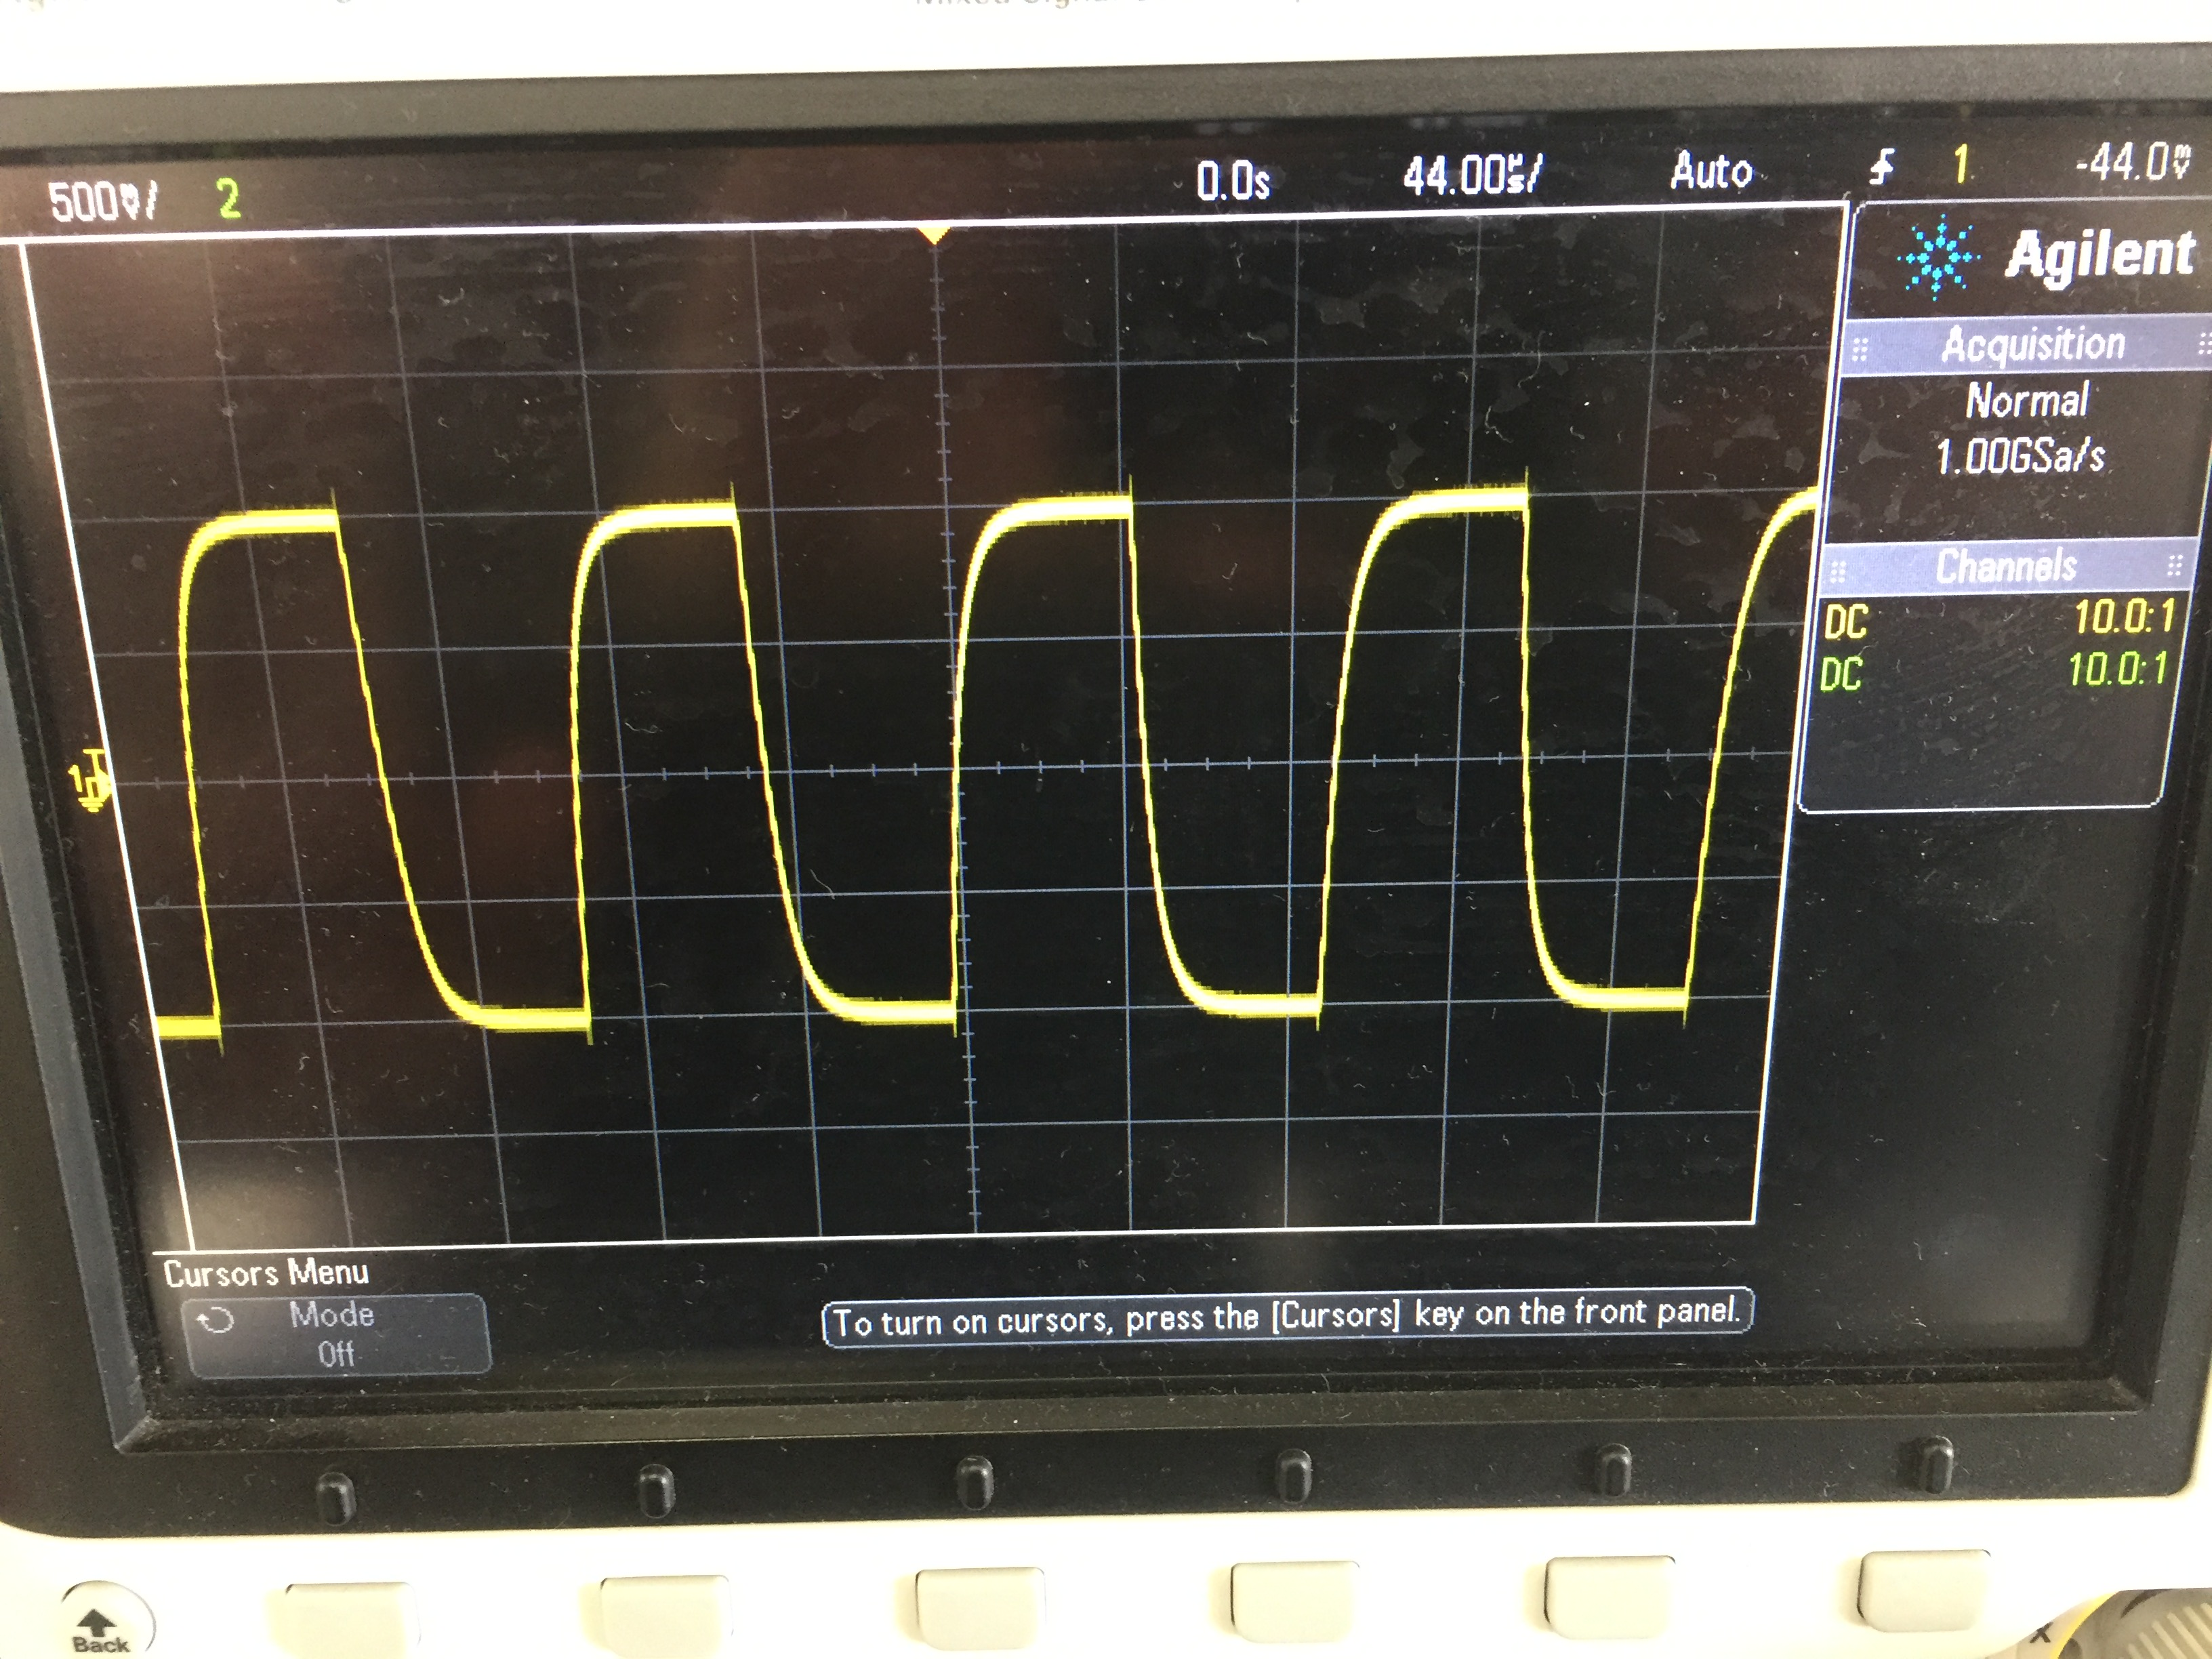
\includegraphics[width=0.7\linewidth]{IMG_6451}
	\label{fig:img6451}
\end{figure}
\begin{figure}[H]
	\centering
	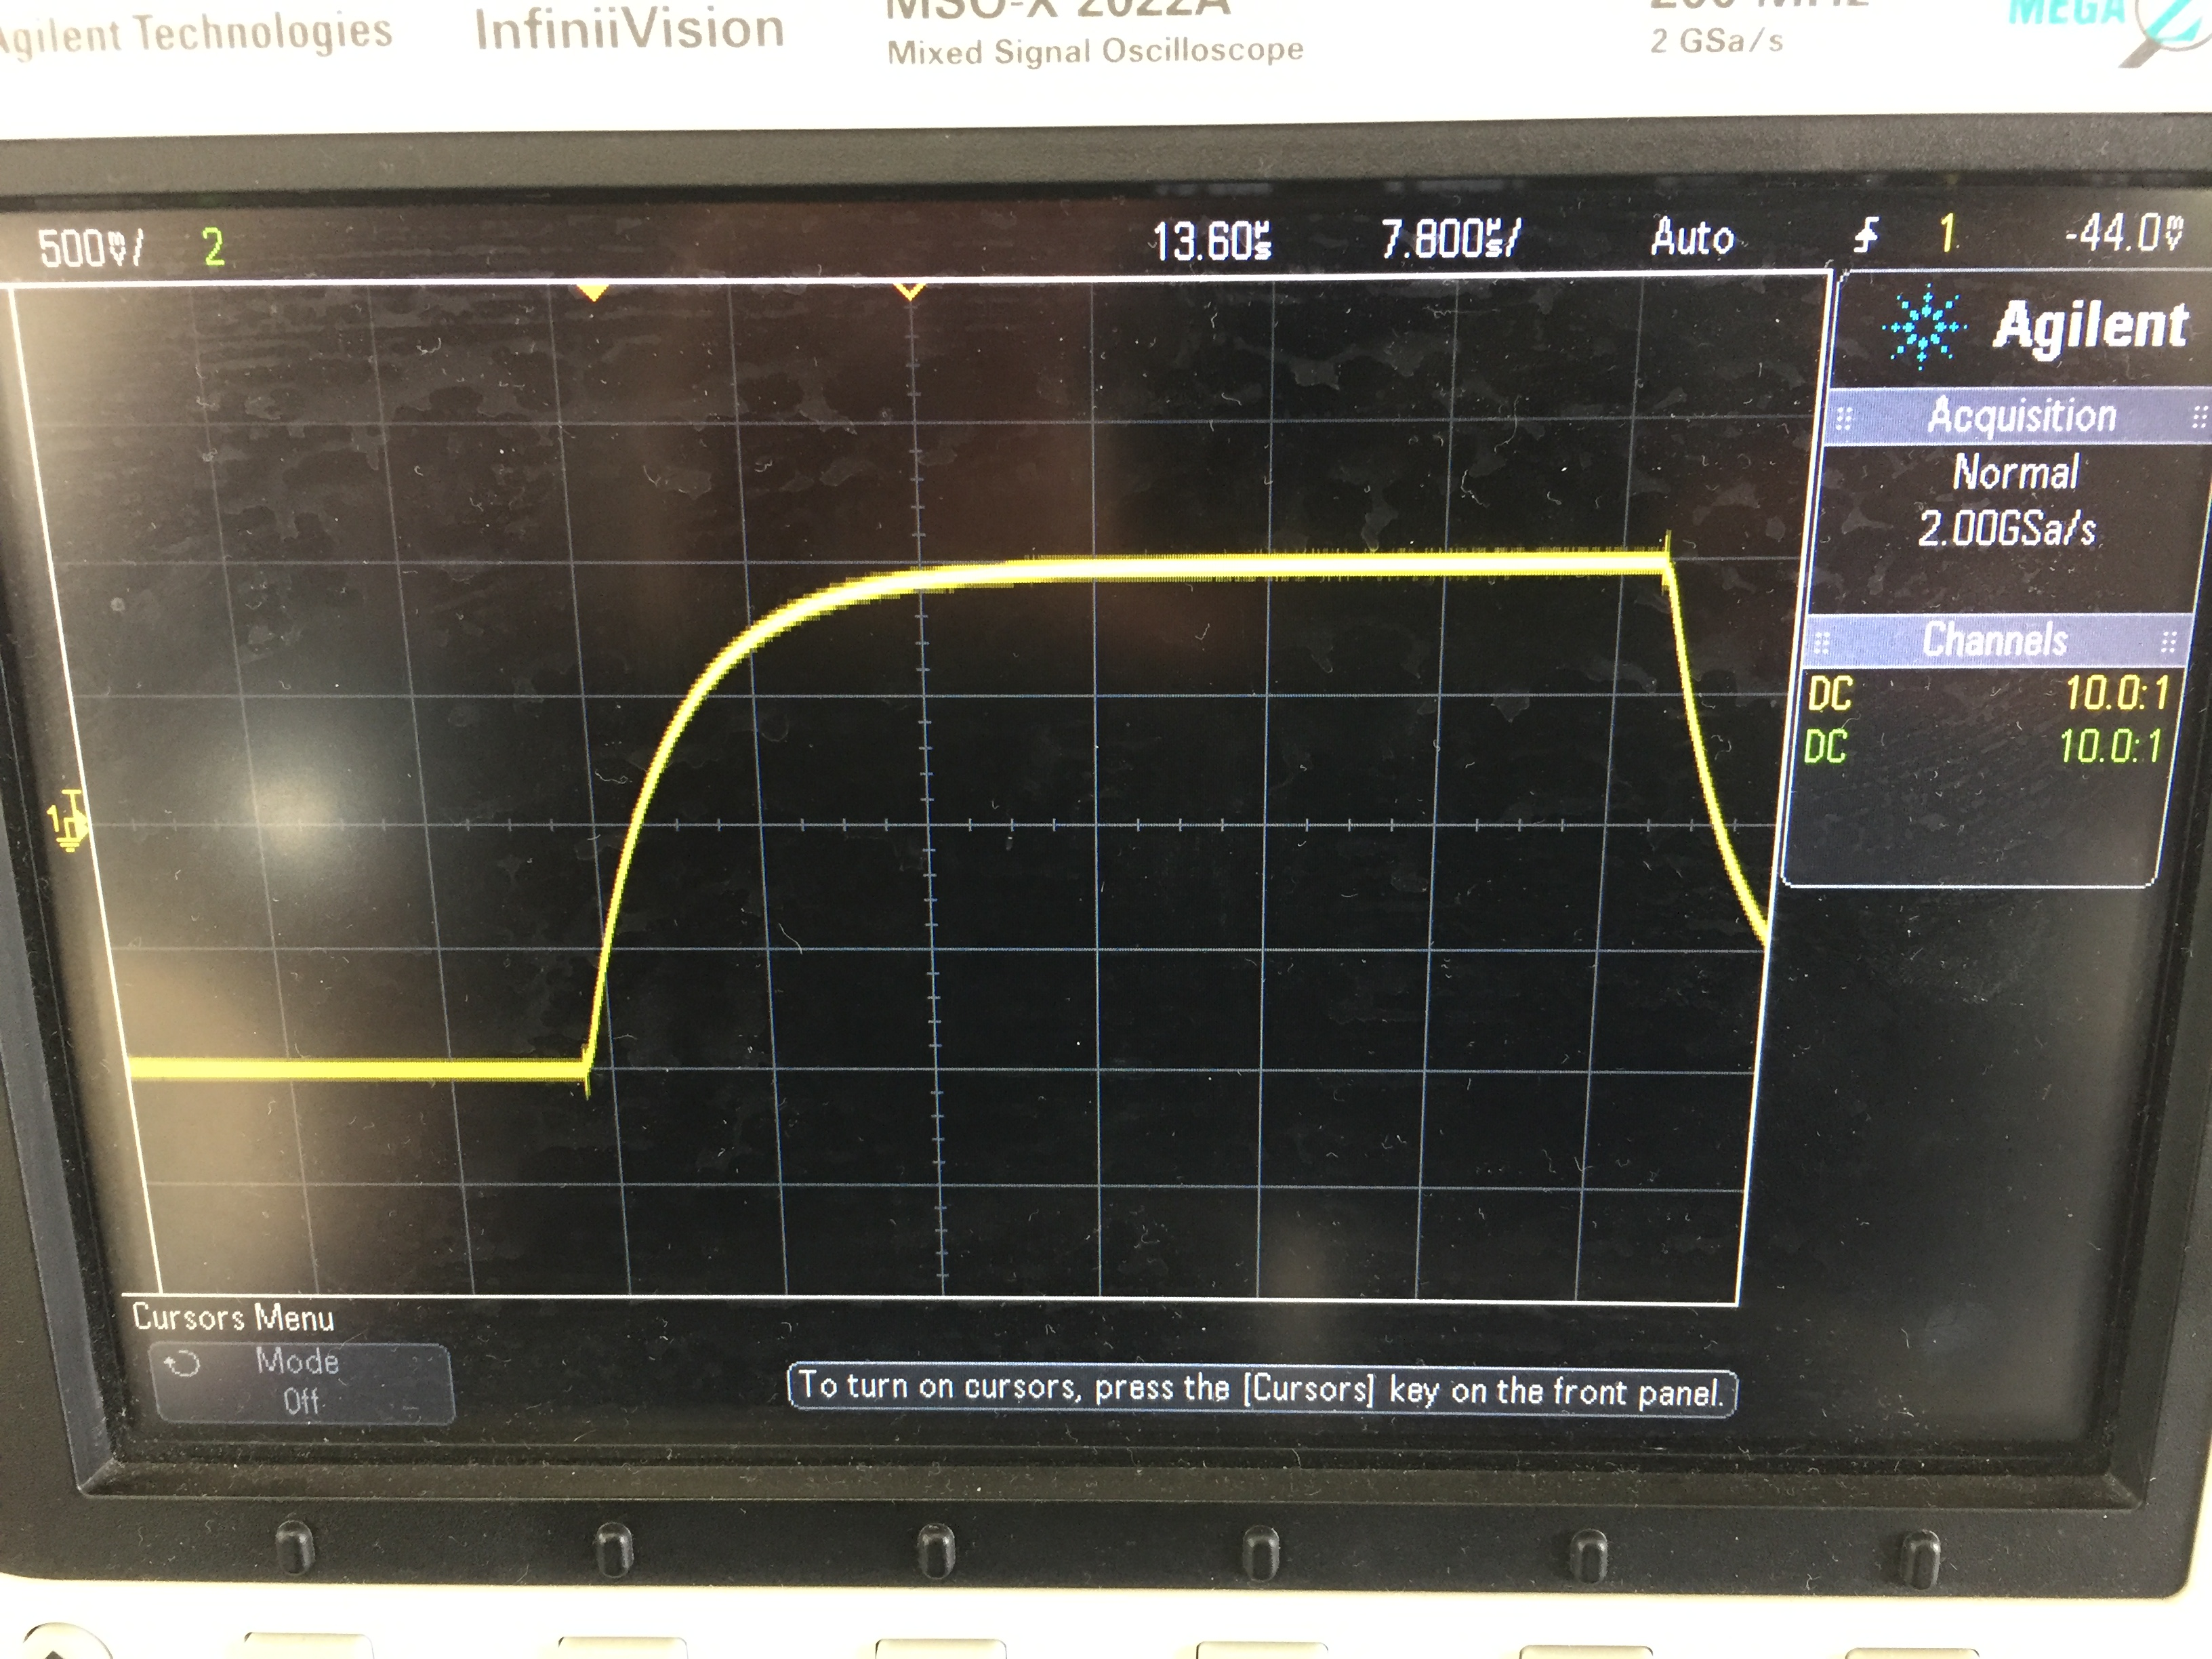
\includegraphics[width=0.7\linewidth]{IMG_6452}
	\label{fig:img6452}
\end{figure}
\begin{figure}[H]
	\centering
	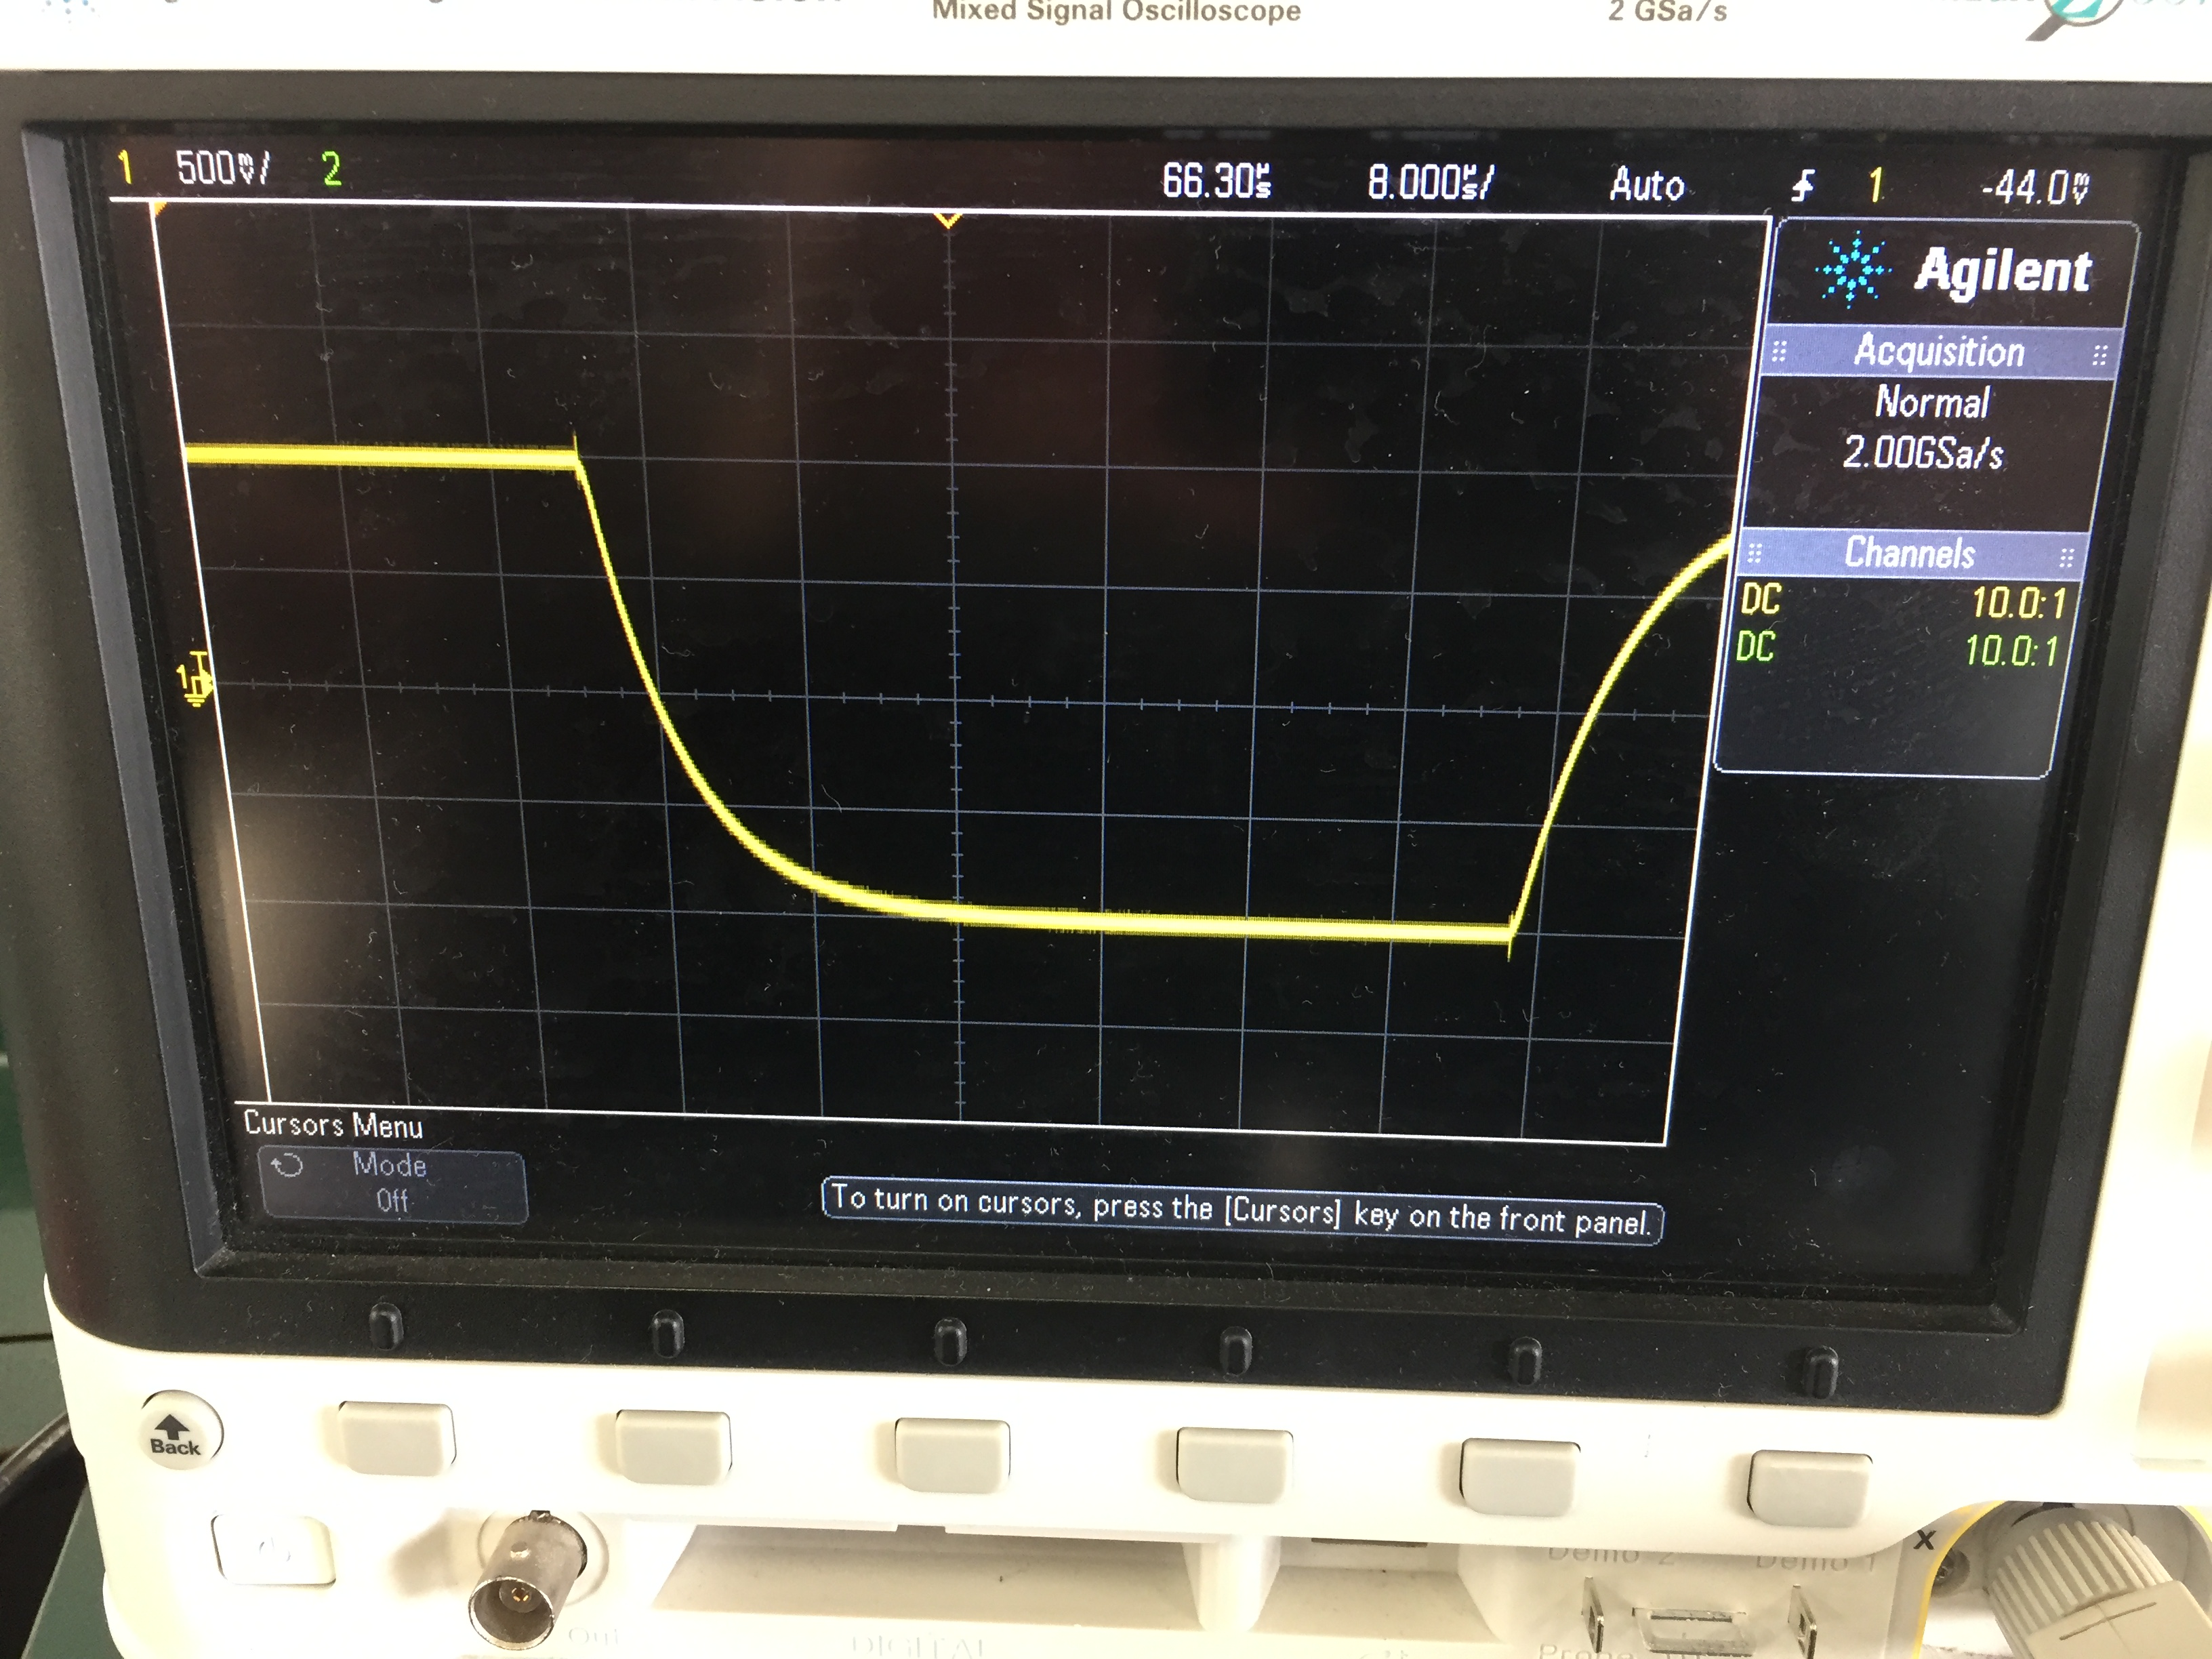
\includegraphics[width=0.7\linewidth]{IMG_6453}
	\label{fig:img6453}
\end{figure}
\begin{figure}[H]
	\centering
	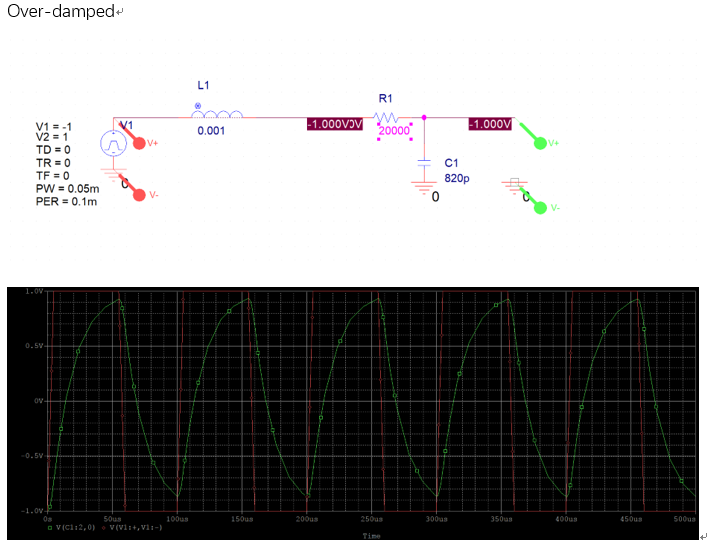
\includegraphics[width=0.7\linewidth]{p3}
	\caption{Over damped}
	\label{fig:p3}
\end{figure}

From the simulation by using Pspice, we find that our output is relatively correct.

In conclusion, this experiment is relatively successful, and I think that the reason why we had a relatively big error in the first part is that we had some trouble when reading 0.1V and 0.9V. If we can have much longer time to do the experiment, we may have a better and more careful reading.
\end{document}